\documentclass[11pt,letterpaper]{article}

\usepackage[margin=1in]{geometry}
\usepackage{amsmath,amssymb}
\usepackage{graphicx}
\usepackage{color}
\usepackage{array}
\usepackage[round]{natbib}

\definecolor{lgray}{gray}{0.52}

\newcommand{\toprule}{\noalign{\hrule height 0.85pt\vspace{2.5pt}}}
\newcommand{\midrule}{\noalign{\vspace{2pt}\hrule height 0.45pt\vspace{2.5pt}}}
\newcommand{\bottomrule}{\noalign{\vspace{2pt}\hrule height 0.85pt}}

% Continuous left-margin line-reference numbers across all pages for review
\newcounter{msline}
\AddToHook{shipout/foreground}{%
  \put(0.56in,-1.12in){%
    \vbox to 0pt{%
      \offinterlineskip
      \count255=0
      \loop\ifnum\count255<46
        \stepcounter{msline}%
        \hbox to 0.26in{\hss\normalfont\scriptsize\color{lgray}\themsline}%
        \vskip 13.8pt
        \advance\count255 by 1
      \repeat
      \vss
    }%
  }%
}

\setlength{\parskip}{0.38em}
\setlength{\parindent}{1.5em}
\setlength{\emergencystretch}{1.6em}
\renewcommand{\arraystretch}{1.18}

\title{\textbf{Cultivation and depensation in a six-species size-spectrum model with external cod recruitment}}

\author{
  Gustav Delius\\[0.3em]
  \small Department of Mathematics, University of York, York YO10 5DD, United Kingdom\\[0.2em]
  \small Running head: \emph{Cultivation and Depensation in a Six-Species Size Spectrum}
}

\date{}

\begin{document}
\maketitle

\begin{abstract}
\noindent
Under one illustrative parameterization of a six-species continental-shelf size-spectrum model with external cod recruitment, numerical analyses demonstrate coexisting locally asymptotically stable high- and low-cod equilibria at zero directed cod fishing. Inspired qualitatively by boreal--temperate gadoid--forage communities of the Northwest Atlantic---where post-collapse stock trajectories have diverged sharply across regions---we formulate a physiologically structured community comprising three pelagic planktivores (capelin-, herring-, and mackerel-like guilds), a demersal ambush mesopredator (sculpin-like), a benthic flatfish competitor (plaice-like), and an apex gadoid (cod-like) in \texttt{mizer} (\texttt{3.4.0.9003}). Holding all biological, trophic-overlap, resource, and non-cod fishing parameters fixed, local linearization of the 727-dimensional consumer--resource ordinary differential equation system at zero cod effort ($E_{\mathrm{cod}} = 0\text{ yr}^{-1}$) identifies a cultivated high-cod fixed point ($\mathrm{SSB}_{\mathrm{cod}} = 1018.2\text{ kt}$, leading eigenvalue $\max\operatorname{Re}(\lambda) = -0.1809\text{ yr}^{-1}$) and a depensatory forage-dominated fixed point ($\mathrm{SSB}_{\mathrm{cod}} = 15.8\text{ kt}$, $\max\operatorname{Re}(\lambda) = -0.0084\text{ yr}^{-1}$), separated by an unstable saddle equilibrium ($\mathrm{SSB}_{\mathrm{cod}} = 42.1\text{ kt}$, $\lambda_+ = +0.0081\text{ yr}^{-1}$). While positive remnant persistence in the low state reflects an imposed open-population cod recruitment flux ($1.1\%$ of calibrated recruitment, or $13.5\%$ in the low state), removing this external input preserves bistability and shifts the lower attractor to cod extinction (invasion $R_0 = 0.82 < 1$). Cumulative mortality-to-growth hazard across $0.001$--$15\text{ g}$ rises from $0.19$ to $2.82$ ($88.7\%$ direct predation led by mackerel, herring, and sculpin; $0.9\%$ growth slowdown alone; $10.4\%$ predation--growth synergy), cutting stationary cohort survival $14.0$-fold ($83.1\%$ to $6.0\%$). Matched six-gear policy experiments show that sparing capelin while thinning herring, mackerel, and sculpin accelerates cod rebuilding, that rebuilding trades off lower aggregate tonnage against gadoid recovery, and that rigid fixed-duration pulses fail under incidental cod fishing $\ge 0.010\text{ yr}^{-1}$ or finer size grids unless replaced by a state-dependent feedback control rule. Structural sweeps confirm that bistability is conditional, disappearing under weaker larval overlap, symmetric fish-larval interactions, wider feeding kernels, stronger cod recruitment compensation, fast resource turnover, or external recruitment $\ge 1.5\%$.

\vspace{0.45em}
\noindent\textbf{Keywords:} cultivation--depensation, alternative stable states, hysteresis, size-spectrum modelling, \texttt{mizer}, Atlantic cod (\emph{Gadus morhua}), forage fish, harvest control rules.
\end{abstract}

\section{Introduction}

Large piscivorous groundfishes hatch at body masses roughly four to seven orders of magnitude smaller than the adult sizes at which they dominate continental-shelf food webs \citep{walters2001cultivation,andersen2019fish}. Throughout egg, larval, and newly settled juvenile stages, young piscivores traverse body-size intervals where small pelagic planktivores and demersal mesopredators---the principal prey of adult piscivores---act instead as competitors for plankton and direct predators on ichthyoplankton and $0$-group settlers. \citet{walters2001cultivation} termed this ontogenetic role reversal \emph{cultivation--depensation}: abundant adult predators ``cultivate'' survival of their own juveniles by cropping smaller-bodied forage and mesopredator guilds, whereas severe depletion of adult predators releases those guilds to establish an early-life demographic bottleneck (emergent depensation) that can impede recovery after directed fishing ceases.

Northwest Atlantic cod (\emph{Gadus morhua}) ecosystems motivated much of the empirical debate surrounding cultivation--depensation following the early-1990s groundfish collapses driven by prolonged overexploitation \citep{hutchings1994what,myers1997why,shelton2006fishing,lilly2013review}, yet subsequent decades demonstrated that Northwest Atlantic stocks did \emph{not} follow a single uniform post-moratorium trajectory. In the southern Gulf of St.~Lawrence (Northwest Atlantic Fisheries Organization [NAFO] Division~4T), \citet{swain2000pelagic} documented a strong negative relationship between pelagic herring (\emph{Clupea harengus}) and mackerel (\emph{Scomber scombrus}) biomass and cod recruitment rate per unit spawning stock biomass (SSB) during the 1970s--1990s, while later virtual population analyses attributed ongoing decline and projected extirpation risk primarily to elevated adult cod natural mortality \citep{swain2008predicted}. On the eastern Scotian Shelf (NAFO Div.~4VsW), groundfish collapse coincided with an approximately nine-fold increase in research-vessel survey biomass indices of small pelagic fishes and benthic macroinvertebrates during the 1990s and early 2000s \citep{frank2005trophic,bundy2005can}, followed by signs of resource limitation within the expanded forage complex and partial benthic return \citep{frank2011transient}. By contrast, in NAFO Divisions~2J3KL off Newfoundland and Labrador, Northern cod did not remain trapped at $1\%$--$5\%$ of historical biomass under an unbroken 34-year closure: inshore fisheries operated in most post-1992 years, Northern cod SSB rebuilt substantially during 2010--2016 to reach $524\text{ kt}$ ($95\%$ confidence interval [CI]: $404$--$678\text{ kt}$; age-$5+$ $F = 0.020\text{ yr}^{-1}$ and $M = 0.32\text{ yr}^{-1}$ in 2024) by 2025 before plateauing \citep{dfo2025cod}, and Fisheries and Oceans Canada (DFO) ended the commercial moratorium on 26~June~2024 \citep{dfo2024reopen,dfo2025cod}. Moreover, NAFO Div.~2J+3KL capelin (\emph{Mallotus villosus}) collapsed in 1991 and remained persistently depleted relative to pre-collapse levels---with a 2024 spring acoustic biomass index of $647\text{ kt}$ ($90\%$ CI: $408$--$1111\text{ kt}$ in text; $1982$--$1990$ median $3697\text{ kt}$; $1991$--$2023$ median $202\text{ kt}$)---where capelin availability positively supports Northern cod condition and survival \citep{rose2002capelin,dfo2025capelin,dfo2025cod}. Likewise, the northern contingent of Atlantic mackerel (NAFO Subareas~3 and~4) remained in DFO's Critical Zone in July~2026 with its commercial fishery closed \citep{dfo2026mackerel}.

This empirical divergence underscores why a deterministic food-web mechanism should not be conflated with a geographic stock reconstruction or used directly to prescribe forage-fish culling in nature \citep{pikitch2014global,garcia2012reconsidering}. Even in single-species age- or size-structured models, compensatory stock--recruitment alone guarantees neither rapid rebuilding nor a unique globally stable equilibrium once stage-specific natural mortality, somatic growth, maternal effects, or fishing selectivity vary; conversely, demonstrating that one food-web configuration produces bistability establishes conditional sufficiency under stated assumptions, not empirical necessity where productivity regimes or adult mortality have shifted \citep{shelton2006fishing,swain2008predicted,lilly2013review}.

From a theoretical perspective, pioneering stage-structured bioenergetic models have shown how ontogenetic diet shifts and prey size truncation can generate alternative attractors in two-species cod--clupeid systems \citep{vanleeuwen2008how,gardmark2015regime}, while continuous multispecies size-spectrum models typically exhibit damped trophic cascades around a unique interior attractor when fishing mortality is varied \citep{andersen2010damped,datta2011stability,andersen2019fish}. Extending cultivation--depensation analysis into a continuous six-species, multi-fleet size-spectrum framework adds three specific mechanistic capabilities beyond two-species stage models:
\begin{enumerate}
  \item \textbf{Predator-resolved demographic hazard across continuous body mass:} Along a stationary size spectrum, cohort survival from hatch weight $w_0$ to upper size $w_1$ obeys
  \begin{equation}
    S(w_0 \to w_1) = \exp\!\big(-H(w_0, w_1)\big), \qquad
    H(w_0, w_1) = \int_{w_0}^{w_1} \frac{\mu(w)}{g(w)}\,\mathrm{d}w,
    \label{eq:survival}
  \end{equation}
  where $\mu(w)$ is instantaneous mortality and $g(w)$ is somatic growth rate (whereas along non-stationary trajectories, survival must be integrated along time-dependent growth characteristics $\mathrm{d}w/\mathrm{d}t = g(w,t)$). Resolving $\mu(w)$ across multiple pelagic and benthic predators separates ichthyoplankton predation by clupeids/scombrids, post-settlement predation by demersal cottids, and food-limited growth slowdown within eq.~\eqref{eq:survival}, while accounting for opposing adult feeding changes at larger body sizes.
  \item \textbf{Multi-dimensional basin geometry vs.\ scalar biomass thresholds:} In a high-dimensional consumer--resource state space, recovery depends on the joint size distribution of predators, prey, and resources rather than scalar gadoid SSB alone, allowing direct comparison between unstable saddle fixed points, path-specific state-space chords, and equal-SSB states with contrasting prey communities.
  \item \textbf{Guild-selective fishing, incidental bycatch, and feedback control:} Resolving separate size-selective fleets for small boreal planktivores (capelin), larger clupeids/scombrids (herring and mackerel), benthic mesopredators (sculpins), flatfish, and juvenile/adult cod bycatch tests when selective predator thinning helps or fails, how aggregate yield trades off against gadoid rebuilding, and why observation-based feedback rules differ from fixed-duration harvest pulses.
\end{enumerate}

Here we construct an illustrative six-species continental-shelf size-spectrum model in \texttt{mizer} \citep{scott2014mizer,mizer2026package} with synthetic reference biomass targets and an explicit open-population cod recruitment input---motivated conceptually by inshore spawning aggregations such as Smith Sound, Trinity Bay \citep{rose2003monitoring,rose2011isolation}, but formulated mathematically as a non-spatial boundary flux---to investigate four questions: (1)~Does the discretized consumer--resource system possess coexisting locally stable high- and low-cod fixed points at $E_{\mathrm{cod}} = 0$, and how sensitive are these equilibria and eigenvalues to numerical solver, time-step, and size-grid choices? (2)~How do direct predation, resource-mediated growth changes, and adult reproductive output combine to determine net reproductive ratio $R_0$ across regimes? (3)~How do basin boundaries, matched six-gear harvest controls, capelin sparing, cod bycatch, and noisy feedback triggers govern transitions back to the high-cod attractor? (4)~Across what parameter region of external recruitment, trophic overlap, feeding-kernel breadth, recruitment compensation, and resource turnover does bistability persist or vanish?

\section{Materials and Methods}

\subsection{Continuous Size-Spectrum Formulation and Exact Executed Rates}

We implement the six-species consumer--resource system in the R package \texttt{mizer} version \texttt{3.4.0.9003} (\texttt{defaults\_edition = 1}, commit \texttt{e2500836}; \citealt{scott2014mizer,andersen2019fish,mizer2026package}). All equations and constants below are verified programmatically against the executed \texttt{MizerParams} objects in \texttt{models/\allowbreak methods\_audit.json}.

For each consumer guild $i \in \{1,\dots,6\}$, the number density $N_i(w,t)$ ($\text{individuals}\cdot\text{g}^{-1}$) is resolved on a logarithmic consumer grid of $\texttt{no\_w} = 100$ bins spanning $w \in [w_0, w_{\max,\mathrm{grid}}]$ with $w_0 = 10^{-3}\text{ g}$ and $w_{\max,\mathrm{grid}} = 22\,500\text{ g}$. Under \texttt{mizer} edition~1 defaults, each guild's numerical upper support is $w_{\max,i} = 1.5\, w_{\infty,i}$ ($75\text{ g}$ for capelin up to $22\,500\text{ g}$ for cod), whereas somatic growth reaches zero at asymptotic mass $w_{\infty,i}$ (\texttt{w\_repro\_max}). Within $w \in [w_0, w_{\max,i}]$, $N_i(w,t)$ satisfies the McKendrick--von Foerster conservation equation
\begin{equation}
  \frac{\partial N_i(w,t)}{\partial t} + \frac{\partial \big[g_i(w,t)\,N_i(w,t)\big]}{\partial w} = -\mu_i(w,t)\,N_i(w,t),
  \label{eq:mvf}
\end{equation}
with boundary flux $g_i(w_0,t)\,N_i(w_0,t) = R_{\mathrm{dd},i}(t)$ at $w_0$.

Consumers coupled to the lower food web graze on an idealized shared resource spectrum $N_R(w,t)$ defined on the extended logarithmic grid $\texttt{w\_full}$ of $222$ bins spanning $[8.70 \times 10^{-13}, 22\,500]\text{ g}$. Resource bins follow size-specific semichemostat dynamics:
\begin{equation}
  \frac{\partial N_R(w,t)}{\partial t} = r_R(w)\,\big[K_R(w) - N_R(w,t)\big] - \mu_{p,R}(w,t)\,N_R(w,t),
  \label{eq:resource}
\end{equation}
where intrinsic turnover follows \texttt{mizer}'s allometric power law $r_R(w) = r_{pp}\, w^{n_R - 1} = 10\, w^{-1/3}\text{ yr}^{-1}$ ($r_{pp} = 10$, $n_R = 2/3$). Resource carrying capacity $K_R(w)$ (\texttt{cc\_pp}) is positive on the $176$ bins strictly below $w_{\mathrm{cut},R} = 10\text{ g}$ (initialized from $\kappa\, w^{-\lambda}$ with $\kappa = 2.8 \times 10^{11}\text{ g}^{\lambda-1}$ and $\lambda = 2.08$, then balanced at calibration steady state via $K_R(w) = N_R^*(w)[1 + \mu_{p,R}^*(w)/r_R(w)]$) and identically zero on the $46$ bins with $w \ge 10\text{ g}$. Biologically, $N_R(w,t)$ represents a combined continuum of pelagic mesozooplankton, euphausiids, and small benthic invertebrates below $10\text{ g}$; treating pelagic and benthic prey below $10\text{ g}$ as a single shared pool is a structural simplification examined in Section~\ref{sec:discussion}.

Predator size selection follows the lognormal mass-ratio kernel
\begin{equation}
  \phi_i(w, w_p) = \exp\!\left[-\frac{\big(\ln[w / (\beta_i w_p)]\big)^2}{2\sigma_i^2}\right],
  \label{eq:kernel}
\end{equation}
with preferred predator-to-prey mass ratio $\beta_i$ and log-width $\sigma_i$. Rather than imposing a hard size cutoff, eq.~\eqref{eq:kernel} concentrates $95\%$ of kernel weight across $w_p / w \in [\beta_i^{-1}\exp(-1.96\sigma_i),\allowbreak\, \beta_i^{-1}\exp(+1.96\sigma_i)]$ (e.g., $5.36\times 10^{-6}$ to $2.98\times 10^{-2}$ for herring, so a $250\text{ g}$ herring concentrates $95\%$ of its kernel across $1.3\text{ mg}$--$7.5\text{ g}$ prey with smooth tails beyond; \texttt{methods\_\allowbreak audit.json}). Volumetric food encounter rate is
\begin{equation}
  \mathcal{E}_i(w,t) = \gamma_i w^{q_i} \int \phi_i(w, w_p)\,\left[N_R(w_p,t) + \sum_{j=1}^{6} \theta_{ij}\,N_j(w_p,t)\right] w_p\,\mathrm{d}w_p,
  \label{eq:encounter}
\end{equation}
where $\gamma_i w^{q_i}$ is search volume with scale-invariant exponent $q_i = n_i + \lambda - 2 = 2/3 + 2.08 - 2 \approx 0.7467$ for all species, and $\theta_{ij} \in [0,1]$ is the dimensionless inter-guild interaction coefficient. Feeding level follows a Type~II functional response $f_i(w,t) = \mathcal{E}_i(w,t) / [\mathcal{E}_i(w,t) + h_i w^{n_i}]$ with maximum intake scaling exponent $n_i = 2/3$. Assimilated intake $\alpha f_i(w,t) h_i w^{n_i}$ ($\alpha = 0.6$), minus metabolic maintenance $k_{s,i} w^{p_i}$ with exponent $p_i = 0.7$, provides net energy $E_{r,i}(w,t) = \max\{0,\, \alpha f_i(w,t) h_i w^{n_i} - k_{s,i} w^{p_i}\}$, which is partitioned by the standard \texttt{mizer} maturity/allocation schedule $\psi_i(w)$ between somatic growth $g_i(w,t)$ (vanishing at $w \ge w_{\infty,i}$) and reproductive energy rate $e_{r,i}(w,t)$ \citep{scott2014mizer,andersen2019fish}.

Predation mortality rate inflicted on fish prey $j$ (or resource $R$, with $\theta_{iR} = 1$) at mass $w_p$ is
\begin{equation}
  \mu_{p,j}(w_p,t) = \sum_{i=1}^{6} \theta_{ij} \int \phi_i(w, w_p)\,\big[1 - f_i(w,t)\big]\,\gamma_i w^{q_i}\,N_i(w,t)\,\mathrm{d}w,
  \label{eq:predmort}
\end{equation}
and total consumer mortality is $\mu_j(w,t) = \mu_{\mathrm{ext},j}(w) + \mu_{p,j}(w,t) + F_j(w,t)$. Because guild-specific constants $z_{0,j}$ are supplied under edition~1 with \texttt{z\_ext = 0}, background external mortality is size-independent across all consumer bins, $\mu_{\mathrm{ext},j}(w) = z_{0,j}$ (Table~\ref{tab:species}A). Instantaneous fishing mortality on species $j$ at mass $w$ sums across commercial gears $g$:
\begin{equation}
  F_j(w,t) = \sum_{g} Q_{g,j}\,E_g(t)\,S_{g,j}(w),
  \label{eq:fishing}
\end{equation}
where $E_g(t)$ ($\text{yr}^{-1}$) is nominal fleet effort, $Q_{g,j}$ is dimensionless gear--species catchability (setting the realized mortality scale per unit effort), and $S_{g,j}(w) \in [0,1]$ is logistic length selectivity (\texttt{sigmoid\_length} parameterized by $L_{50}$ and $L_{25}$ via $w = a_j L^{b_j}$; Table~\ref{tab:gears}).

\subsection{Synthetic Community Parameterization, Provenance, and Open Recruitment}

The six guilds represent idealized functional archetypes inspired by boreal--temperate continental-shelf communities (Table~\ref{tab:species}A; full parameter provenance ledger in \texttt{paper/provenance\_ledger.md}): (1)~small boreal planktivore (\texttt{Capelin}, $w_\infty = 50\text{ g}$, $\beta = 2000$), (2)~medium clupeid planktivore (\texttt{Herring}, $w_\infty = 380\text{ g}$, $\beta = 2500$), (3)~fast pelagic planktivore/piscivore (\texttt{Mackerel}, $w_\infty = 850\text{ g}$, $\beta = 350$), (4)~demersal ambush mesopredator (\texttt{Sculpin}, $w_\infty = 1100\text{ g}$, $\beta = 65$), (5)~benthic flatfish competitor (\texttt{Plaice}, $w_\infty = 2600\text{ g}$, $\beta = 220$), and (6)~large apex gadoid (\texttt{Cod}, $w_\infty = 15\,000\text{ g}$, $w_{\mathrm{mat}} = 850\text{ g}$, $\beta = 60$).

\begin{table}[t!]
\centering
\caption{Guild life-history traits, feeding-kernel parameters, synthetic calibration targets, and internally calibrated bioenergetic/recruitment parameters at $E_{\mathrm{cal}} = (0.15, 0.05, 0.15, 0.22)\text{ yr}^{-1}$. All weight--length conversions use $b_i = 3.0$. Synthetic reference biomasses $B_i^{\mathrm{syn}}$ ($1\text{ kt} = 10^9\text{ g}$, evaluated on $w \ge w_{\mathrm{cut},i}$) are illustrative community targets, not empirical survey estimates.}
\label{tab:species}
\vspace{0.35em}
{\footnotesize
\setlength{\tabcolsep}{5.2pt}
\begin{tabular}{lrrrrrrrrr}
\toprule
\multicolumn{10}{l}{\textbf{A. Imposed life-history traits, feeding kernels, and synthetic cutoff-biomass targets}} \\
\midrule
Guild & $w_\infty$ & $w_{\mathrm{mat}}$ & $k_{\mathrm{vb}}$ & $z_0$ & $\beta_i$ & $\sigma_i$ & $a_i$ & $B_i^{\mathrm{syn}}$ & $w_{\mathrm{cut},i}$ \\
      & (g) & (g) & ($\text{yr}^{-1}$) & ($\text{yr}^{-1}$) & & & ($\text{g cm}^{-3}$) & (kt) & (g) \\
\midrule
Capelin  &    50 &   7 & 0.75 & 0.38 & 2000 & 1.8 & 0.0060 & 520 &  2 \\
Herring  &   380 &  55 & 0.58 & 0.35 & 2500 & 2.2 & 0.0070 & 380 & 10 \\
Mackerel &   850 & 115 & 0.52 & 0.34 &  350 & 1.9 & 0.0080 & 190 & 15 \\
Sculpin  &  1100 &  95 & 0.42 & 0.54 &   65 & 1.6 & 0.0120 & 140 & 15 \\
Plaice   &  2600 & 180 & 0.28 & 0.28 &  220 & 1.7 & 0.0090 & 260 & 20 \\
Cod      & 15000 & 850 & 0.26 & 0.20 &   60 & 1.6 & 0.0085 & 680 & 50 \\
\bottomrule
\end{tabular}

\vspace{0.45em}
\setlength{\tabcolsep}{3.0pt}
\begin{tabular}{@{}lrrrrrrrrr@{}}
\toprule
\multicolumn{10}{@{}l@{}}{\textbf{B. Calibrated bioenergetic rates, Beverton--Holt parameters, and post-subsidy biomasses}} \\
\midrule
Guild & $h_i$ & $\gamma_i$ & $k_{s,i}$ & $r_i$ & $\varepsilon_{\mathrm{repro},i}$ & $R_{\max,i}$ & $B_i^{\mathrm{pre}}$ & $B_i^{\mathrm{post}}$ & $\Delta B_i$ \\
      & ($\text{g}^{1/3}\text{yr}^{-1}$) & ($10^{-11}$) & ($\text{g}^{0.3}\text{yr}^{-1}$) & & & ($\text{yr}^{-1}$) & (kt) & (kt) & (\%) \\
\midrule
Capelin  & 24.20 & 1.42 & 2.72 & 0.88 & $1.70 \times 10^{-3}$ & $8.05 \times 10^{10}$ & 520.0 & 507.3 & $-2.45$ \\
Herring  & 37.35 & 1.75 & 3.92 & 0.88 & $5.72 \times 10^{-4}$ & $1.37 \times 10^{10}$ & 380.0 & 367.0 & $-3.43$ \\
Mackerel & 47.15 & 3.01 & 4.83 & 0.88 & $2.27 \times 10^{-4}$ & $2.65 \times 10^{9}$  & 190.0 & 184.0 & $-3.17$ \\
Sculpin  & 44.76 & 3.91 & 4.61 & 0.88 & $4.81 \times 10^{-4}$ & $3.06 \times 10^{9}$  & 140.0 & 136.0 & $-2.89$ \\
Plaice   & 38.33 & 2.85 & 3.87 & 0.88 & $7.36 \times 10^{-5}$ & $6.41 \times 10^{8}$  & 260.0 & 257.1 & $-1.10$ \\
Cod      & 66.73 & 5.87 & 6.40 & 0.28 & $2.12 \times 10^{-6}$ & $7.43 \times 10^{8}$  & 680.0 & 687.2 & $+1.06$ \\
\bottomrule
\end{tabular}
}
\end{table}

Two structural assumptions shape the baseline parameterization and are subjected to systematic sensitivity sweeps in Section~\ref{sec:sensitivity}. First, the illustrative interaction matrix $\theta_{ij}$ (Table~\ref{tab:inter}) imposes strong asymmetry between predator--cod encounters ($\theta_{i,\mathrm{Cod}} \in [0.45, 1.00]$ for pelagic planktivores and sculpin; $\theta_{\mathrm{Cod},j} \in [0.38, 0.45]$) and weak intra-forage fish predation ($\theta_{ij} \in [0.01, 0.05]$ among non-cod guilds). Because $\theta_{ij}$ is species-constant rather than stage-indexed, actual size selectivity arises through $\phi_i(w, w_p)$: in the low-cod equilibrium, $79.4\%$ of total pre-maturation ($<850\text{ g}$) predation hazard on cod occurs below $15\text{ g}$ and $92.6\%$ occurs below $50\text{ g}$. Second, at calibration steady state we impose Beverton--Holt reproduction levels $r_i = R_{\mathrm{dd},i}^* / R_{\max,i}$ of $r_{\mathrm{prey}} = 0.88$ for the five non-cod guilds and $r_{\mathrm{Cod}} = 0.28$ for cod (reference recruitment elasticity $1 - r_i$ equal to $0.12$ vs.\ $0.72$ prior to external cod input).

\begin{table}[t!]
\centering
\caption{Illustrative inter-guild interaction matrix $\theta_{ij}$ (rows = predators $i$, columns = prey $j$).}
\label{tab:inter}
\vspace{0.35em}
{\small
\setlength{\tabcolsep}{7pt}
\begin{tabular}{lrrrrrr}
\toprule
Predator $\backslash$ Prey & Capelin & Herring & Mackerel & Sculpin & Plaice & Cod \\
\midrule
Capelin  & 0.01 & 0.01 & 0.01 & 0.01 & 0.01 & 0.55 \\
Herring  & 0.02 & 0.01 & 0.01 & 0.01 & 0.02 & 1.00 \\
Mackerel & 0.04 & 0.02 & 0.01 & 0.01 & 0.02 & 1.00 \\
Sculpin  & 0.05 & 0.02 & 0.01 & 0.02 & 0.03 & 0.45 \\
Plaice   & 0.04 & 0.02 & 0.01 & 0.01 & 0.01 & 0.02 \\
Cod      & 0.45 & 0.43 & 0.40 & 0.38 & 0.12 & 0.025 \\
\bottomrule
\end{tabular}
}
\end{table}

Boundary recruitment at $w_0 = 10^{-3}\text{ g}$ combines endogenous Beverton--Holt density dependence with an additive exogenous recruitment input $R_{\mathrm{ext},i}$ (\texttt{r\_refuge} in \texttt{RefugeBevertonHoltRDD}):
\begin{equation}
  R_{\mathrm{dd},i}(t) = \frac{R_{\mathrm{di},i}(t)}{1 + R_{\mathrm{di},i}(t) / R_{\max,i}} + R_{\mathrm{ext},i}, \qquad
  R_{\mathrm{di},i}(t) = \frac{\varepsilon_{\mathrm{repro},i}}{2 w_0} \int_{w_0}^{w_{\max,i}} e_{r,i}(w,t)\,N_i(w,t)\,\mathrm{d}w.
  \label{eq:rdd}
\end{equation}
In the baseline configuration, $R_{\mathrm{ext,Cod}} = 2.290 \times 10^6\text{ recruits yr}^{-1}$ ($1.10\%$ of calibrated cod recruitment at $E_{\mathrm{cal}}$) and $R_{\mathrm{ext},i} = 0$ for all other guilds. Equation~\eqref{eq:rdd} is an open-population boundary assumption---not a mechanistic model of sheltered fjord juvenile survival---because incoming recruits enter at $w_0 = 1\text{ mg}$ and immediately experience the shelf mortality and resource fields. Because $R_{\mathrm{ext,Cod}} > 0$ renders $N_{\mathrm{Cod}} \equiv 0$ non-invariant, persistence of a positive low-cod remnant is imposed by construction; to separate assumed persistence from emergent bistability, Section~\ref{sec:sensitivity} evaluates $R_{\mathrm{ext,Cod}} = 0$, a sweep over $R_{\mathrm{ext,Cod}}/R_{\mathrm{dd,Cod}}^{\mathrm{cal}} \in [0, 0.05]$, nursery export size classes $w_{\mathrm{entry}} \in [0.001, 50]\text{ g}$, and a zero-cod-invariant spawner-linked formulation (\texttt{SaturatingShelterRDD}):
\begin{equation}
  R_{\mathrm{dd},i}^{\mathrm{shelter}}(t) = \frac{R_{\mathrm{di},i}(t)}{1 + R_{\mathrm{di},i}(t) / R_{\max,i}} + \frac{R_{\mathrm{ref,\max},i}\,R_{\mathrm{di},i}(t)}{R_{\mathrm{di},i}(t) + K_{\mathrm{ref},i}},
  \label{eq:shelter}
\end{equation}
which satisfies $R_{\mathrm{dd,Cod}}^{\mathrm{shelter}} = 0$ whenever $R_{\mathrm{di,Cod}} = 0$.

\begin{table}[t!]
\centering
\caption{Fleet structure, logistic length-selectivity parameters ($L_{50}, L_{25}$), catchabilities $Q_{g,j}$, and baseline effort regimes ($E_{\mathrm{hist}}$ vs.\ zero-cod-fishing $E_{\mathrm{mor}}$). In the 4-gear configuration, \texttt{Pelagic} aggregates capelin ($Q = 0.75$, so $E_{\mathrm{pel}} = 0.15\text{ yr}^{-1}$ gives asymptotic $F = 0.1125\text{ yr}^{-1}$), herring ($Q = 1.0$), and mackerel ($Q = 1.0$). In the matched 6-gear extension, \texttt{Capelin\_Gear} and \texttt{Clupeid\_Mackerel} are controlled independently alongside size-selective \texttt{Cod\_Bycatch}.}
\label{tab:gears}
\vspace{0.35em}
{\footnotesize
\setlength{\tabcolsep}{5.2pt}
\begin{tabular}{lllrrrrr}
\toprule
4-Gear Fleet & 6-Gear Extension Fleet & Guild & $L_{50}$ (cm) & $L_{25}$ (cm) & $Q_{g,j}$ & $E_{\mathrm{hist}}$ ($\text{yr}^{-1}$) & $E_{\mathrm{mor}}$ ($\text{yr}^{-1}$) \\
\midrule
Pelagic      & Capelin\_Gear     & Capelin  & 11 &  9 & 0.75 & 0.15 & 0.15 \\
Pelagic      & Clupeid\_Mackerel & Herring  & 20 & 16 & 1.00 & 0.15 & 0.15 \\
Pelagic      & Clupeid\_Mackerel & Mackerel & 25 & 20 & 1.00 & 0.15 & 0.15 \\
Mesopredator & Mesopredator      & Sculpin  & 20 & 16 & 1.00 & 0.05 & 0.05 \\
Flatfish     & Flatfish          & Plaice   & 28 & 23 & 1.00 & 0.15 & 0.15 \\
Cod\_Trawl   & Cod\_Trawl        & Cod      & 52 & 45 & 1.00 & 0.15 & 0.00 \\
---          & Cod\_Bycatch (juv./adult) & Cod & 22 / 52 & 17 / 45 & 1.00 & 0.00 & 0.00 \\
\bottomrule
\end{tabular}
}
\end{table}

\subsection{Calibration, Numerical Solvers, Stability, and Policy Experiments}

Steady-state calibration (\texttt{R/01\_build\_\allowbreak and\_calibrate\_\allowbreak model.R}) was performed at $E_{\mathrm{cal}} = (0.15,\allowbreak\, 0.05,\allowbreak\, 0.15,\allowbreak\, 0.22)\text{ yr}^{-1}$---deliberately selecting $E_{\mathrm{cod}} = 0.22\text{ yr}^{-1}$ near the upper exploited branch so that the reference fished state $E_{\mathrm{hist}}$ ($E_{\mathrm{cod}} = 0.15\text{ yr}^{-1}$) lies well inside the high-cod basin of attraction. Alternating \texttt{matchGrowth()}, \texttt{matchBiomasses()}, \texttt{steadySingleSpecies(\allowbreak ..., keep = "biomass")}, \texttt{setBevertonHolt()}, and \texttt{tuneSteadyState()} matched the synthetic pre-subsidy cutoff-biomass targets $B_i^{\mathrm{syn}}$ to $< 2 \times 10^{-13}\%$ with $\varepsilon_{\mathrm{repro},i} \in [2.12 \times 10^{-6}, 1.70 \times 10^{-3}]$ (Table~\ref{tab:species}B; note $\varepsilon_{\mathrm{repro},i} < 1$ is an internal bioenergetic consistency check, not empirical validation). Adding $R_{\mathrm{ext,Cod}}$ and settling at $E_{\mathrm{cal}}$ shifted cod cutoff biomass by $+1.06\%$ ($687.2\text{ kt}$) and non-cod cutoff biomasses by $-1.10\%$ to $-3.43\%$ (Table~\ref{tab:species}B).

All dynamic projections across \texttt{R/01}--\texttt{R/04} share one canonical time integrator: the second-order trapezoidal backward-differentiation scheme (\texttt{method = "tr\_bdf2"}) with $\Delta t = 0.05\text{ yr}$ under standard first-order upwind size transport (\texttt{second\_order\_w}: \texttt{flux = "upwind"}, \texttt{bin\_average = FALSE}). Reference equilibria were refined via \texttt{findSteadyState()} to a strict convergence tolerance $\texttt{residual\_tol} = 10^{-8}\text{ yr}^{-1}$ and verified using both biomass-weighted and per-capita rate-of-change residuals. Local stability of the discretized ODE system was evaluated with \texttt{getStability()} across finite-difference steps $h \in \{10^{-3}, 10^{-4}, 10^{-5}, 10^{-6}\}$ and discrete-time Jacobian spectral radii (\texttt{getDiscreteStability()}). Under upwind transport, \texttt{getStability()} perturbs $\texttt{n\_fish\_active} = 505$ active consumer bins ($67, 79, 84, 85, 90, 100$ bins for capelin, herring, mackerel, sculpin, plaice, and cod, spanning $w_0$ through $\min\{\#\{w \le w_{\max,i}\} + 1, 100\}$) plus all $222$ resource bins, yielding $\texttt{n\_active} = 727$ eigenvalues \citep{datta2011stability,mizer2026package}. Intervening unstable saddle fixed points were polished via \texttt{findSteadyState(..., solver = "newton")} initialized near straight-chord bisection brackets.

Using relative simulation time $t$ (years), the illustrative collapse-and-closure trajectory ($t \in [0, 61]$) holds $E_{\mathrm{cod}} = 0.15\text{ yr}^{-1}$ on $t \in [0, 3)$, escalates to $0.46\text{ yr}^{-1}$ on $t \in [3, 16)$ and $0.56\text{ yr}^{-1}$ on $t \in [16, 27)$, and closes directed cod fishing ($E_{\mathrm{cod}} = 0$) across $t \in [27, 61]$ while maintaining baseline non-cod efforts ($E_{\mathrm{pel}} = 0.15$, $E_{\mathrm{meso}} = 0.05$, $E_{\mathrm{flat}} = 0.15\text{ yr}^{-1}$). Post-closure policy experiments initialize at $t = 61$ ($\tau = t - 61 \in [0, 40]\text{ yr}$) and are projected for an additional $300\text{ yr}$ ($\tau = 340\text{ yr}$) under constant post-switch efforts to verify asymptotic basin membership directly. Alongside the 4-gear $(E_{\mathrm{pel}}, E_{\mathrm{meso}}, E_{\mathrm{cod}})$ surface, we evaluate 11 matched 6-gear scenarios isolating tapering from cod reopening and capelin sparing from clupeid/mackerel harvest, sweep Phase-I juvenile ($L_{50} = 22\text{ cm}$) and adult ($L_{50} = 52\text{ cm}$) cod bycatch $E_{\mathrm{byc}} \in [0, 0.10]\text{ yr}^{-1}$, and test an annual state-dependent feedback harvest control rule (switching from Phase~I to Phase~II with a $1\text{ yr}$ implementation lag after two consecutive annual survey observations satisfy $\widehat{\mathrm{SSB}}_{\mathrm{cod}} \ge 280\text{ kt}$ under multiplicative lognormal error with $\mathrm{CV} = 0.25$ across $16$ replicates).

\section{Results}

\subsection{Simulated Collapse, Guild Reversal, and Post-Closure Stagnation}

Starting from the high-cod fished steady state at $t = 0$ ($\mathrm{SSB}_{\mathrm{cod}} = 776.3\text{ kt}$; cutoff biomass $824.8\text{ kt}$ above $50\text{ g}$; cod yield $128.5\text{ kt}\cdot\text{yr}^{-1}$), escalating $E_{\mathrm{cod}}$ to $0.46$ and $0.56\text{ yr}^{-1}$ across $t \in [3, 27)$ drives cod SSB down by $99.4\%$ to $4.56\text{ kt}$ at $t = 27\text{ yr}$ (Fig.~\ref{fig:history}A). Predation release triggers a community-wide guild expansion: combined cutoff biomass of capelin, herring, mackerel, and sculpin increases $7.35$-fold relative to the $E_{\mathrm{cod}} = 0.15\text{ yr}^{-1}$ equilibrium (from $751.4\text{ kt}$ to $5524.6\text{ kt}$ once settled, or $16.14$-fold relative to the $342.3\text{ kt}$ zero-cod-fishing cultivated state). Closing directed cod fishing completely at $t = 27\text{ yr}$ ($E_{\mathrm{cod}} = 0$; Fig.~\ref{fig:history}B) fails to restore gadoid dominance: across the 34-year closure ($t = 27$--$61\text{ yr}$), cod SSB rises only from $4.56\text{ kt}$ to $9.17\text{ kt}$ ($9.35\text{ kt}$ cutoff biomass), slowly approaching an interior low-cod equilibrium under unchanged biological parameters.

\begin{figure}[t!]
  \centering
  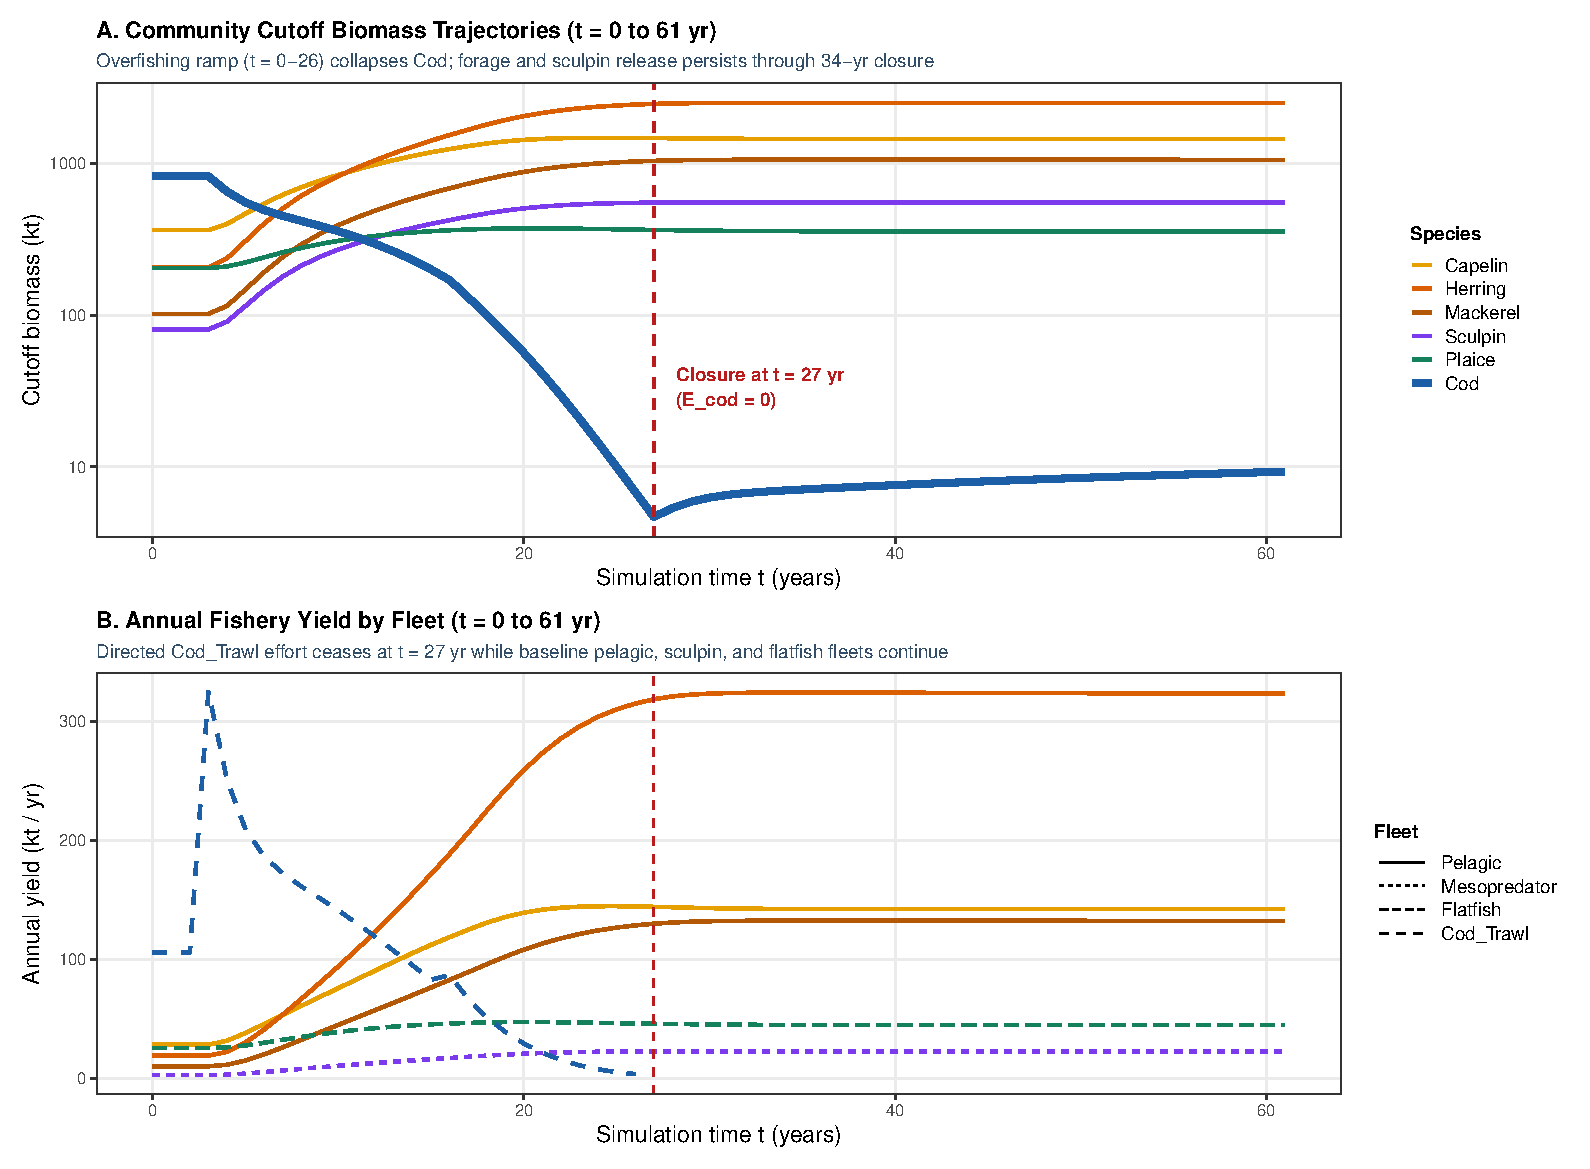
\includegraphics[width=0.96\textwidth]{figures/fig1_collapse_moratorium.pdf}
  \caption{Illustrative groundfish collapse ($t = 0$--$26\text{ yr}$) and 34-year directed-cod closure ($t = 27$--$61\text{ yr}$) in relative simulation time (\texttt{tr\_bdf2}, $\Delta t = 0.05\text{ yr}$). \textbf{(A)} Biomass trajectories of all six guilds above their respective size cutoffs $w_{\mathrm{cut},i}$ (Table~\ref{tab:species}A), highlighting cod. \textbf{(B)} Projected annual landings by commercial gear. Setting $E_{\mathrm{cod}} = 0$ at $t = 27\text{ yr}$ leaves cod at $9.17\text{ kt}$ SSB by $t = 61\text{ yr}$.}
  \label{fig:history}
\end{figure}

\subsection{Coexisting Steady States, Unstable Saddles, and Path-Specific Basins}

Refining the discretized system to $\texttt{residual\_tol} = 10^{-8}\text{ yr}^{-1}$ confirms coexisting locally asymptotically stable high- and low-cod fixed points at both $E_{\mathrm{cod}} = 0$ and $E_{\mathrm{cod}} = 0.15\text{ yr}^{-1}$ (Table~\ref{tab:equilibria}; Fig.~\ref{fig:spectra}). Notice that the $E_{\mathrm{cod}} = 0$ states represent \emph{zero-cod-fishing} communities in which baseline pelagic, mesopredator, and flatfish fishing remain active (Table~\ref{tab:gears}), not an unexploited ecosystem.

At $E_{\mathrm{cod}} = 0\text{ yr}^{-1}$, the cultivated equilibrium maintains $\mathrm{SSB}_{\mathrm{cod}} = 1018.2\text{ kt}$ ($1063.0\text{ kt}$ cutoff biomass) and crops herring ($33.5\text{ kt}$ SSB), mackerel ($17.6\text{ kt}$), sculpin ($16.9\text{ kt}$), and capelin ($168.6\text{ kt}$), with biomass-weighted residual $1.49 \times 10^{-9}\text{ yr}^{-1}$ and all $727$ Jacobian eigenvalues strictly in the open left half-plane ($\max\operatorname{Re}(\lambda) = -0.1809\text{ yr}^{-1}$, damped oscillation period $19.1\text{ yr}$; invariant to seven significant digits across $h \in [10^{-6}, 10^{-3}]$). (In \texttt{cod\_high\_f0}, four ultra-trace cod bins above $9.5\text{ kg}$ holding $< 0.04\text{ g}$ total biomass have $g(w) = 0$ due to adult food limitation and thus per-capita decay $-z_0 = -0.20\text{ yr}^{-1}$ while contributing $< 4 \times 10^{-11}$ to biomass drift.) Under identical parameters, the depensatory $E_{\mathrm{cod}} = 0$ equilibrium holds $\mathrm{SSB}_{\mathrm{cod}} = 15.8\text{ kt}$ ($15.9\text{ kt}$ cutoff biomass; biomass residual $2.28 \times 10^{-9}\text{ yr}^{-1}$, per-capita residual $8.59 \times 10^{-7}\text{ yr}^{-1}$) beneath an expanded dome of herring ($2313.3\text{ kt}$ SSB), capelin ($1373.9\text{ kt}$), mackerel ($968.0\text{ kt}$), and sculpin ($490.7\text{ kt}$), with $\max\operatorname{Re}(\lambda) = -0.00841\text{ yr}^{-1}$ (real leading eigenvalue; local relaxation timescale $\sim 119\text{ yr}$). Discrete-time spectral radii remain strictly below unity at all reference equilibria across $\Delta t \in \{0.05, 0.10, 0.20\}\text{ yr}$ ($0.9851$, $0.9913$, and $0.9996$ at $\Delta t = 0.05\text{ yr}$).

\begin{table}[t!]
\centering
\caption{Refined steady-state spawning stock biomasses (kt), cod cutoff biomasses ($w \ge 50\text{ g}$), convergence residuals, and 727-dimensional Jacobian spectra (\texttt{getStability()}, $h = 10^{-5}$) for the four stable fixed points and two Newton-polished unstable saddle equilibria.}
\label{tab:equilibria}
\vspace{0.35em}
{\footnotesize
\setlength{\tabcolsep}{3.8pt}
\begin{tabular}{lrrrrrr}
\toprule
Metric & Cultivated & Saddle & Depensatory & Fished High & Saddle & Fished Low \\
       & ($E_{\mathrm{cod}}=0$) & ($E_{\mathrm{cod}}=0$) & ($E_{\mathrm{cod}}=0$) & ($E_{\mathrm{cod}}=0.15$) & ($E_{\mathrm{cod}}=0.15$) & ($E_{\mathrm{cod}}=0.15$) \\
\midrule
Capelin SSB (kt)        &  168.6 & 1369.0 & 1373.9 &  297.4 & 1095.6 & 1375.7 \\
Herring SSB (kt)        &   33.5 & 2221.7 & 2313.3 &  139.3 & 1207.3 & 2363.6 \\
Mackerel SSB (kt)       &   17.6 &  932.9 &  968.0 &   76.3 &  545.8 &  987.3 \\
Sculpin SSB (kt)        &   16.9 &  480.0 &  490.7 &   59.3 &  329.4 &  496.5 \\
Plaice SSB (kt)         &  109.9 &  324.4 &  323.1 &  182.8 &  321.8 &  322.4 \\
\textbf{Cod SSB (kt)}   & \textbf{1018.2} & \textbf{42.1} & \textbf{15.8} & \textbf{776.3} & \textbf{321.7} & \textbf{1.3} \\
Cod cutoff biomass (kt) & 1063.0 &   42.6 &   15.9 &  824.8 &  338.8 &    1.3 \\
\midrule
Biomass resid.\ ($\text{yr}^{-1}$) & $1.49\times 10^{-9}$ & $3.00\times 10^{-7}$ & $2.28\times 10^{-9}$ & $5.93\times 10^{-9}$ & $1.64\times 10^{-7}$ & $1.81\times 10^{-9}$ \\
Max $\operatorname{Re}(\lambda)$ ($\text{yr}^{-1}$) & $-0.1809$ & $+0.0081$ & $-0.0084$ & $-0.3036$ & $+0.0778$ & $-0.1320$ \\
Unstable modes ($n_+ / 727$) & $0$ & $1$ & $0$ & $0$ & $1$ & $0$ \\
Stability ($N=727$ ODE) & Stable & Saddle & Stable & Stable & Saddle & Stable \\
\bottomrule
\end{tabular}
}
\end{table}

\begin{figure}[t!]
  \centering
  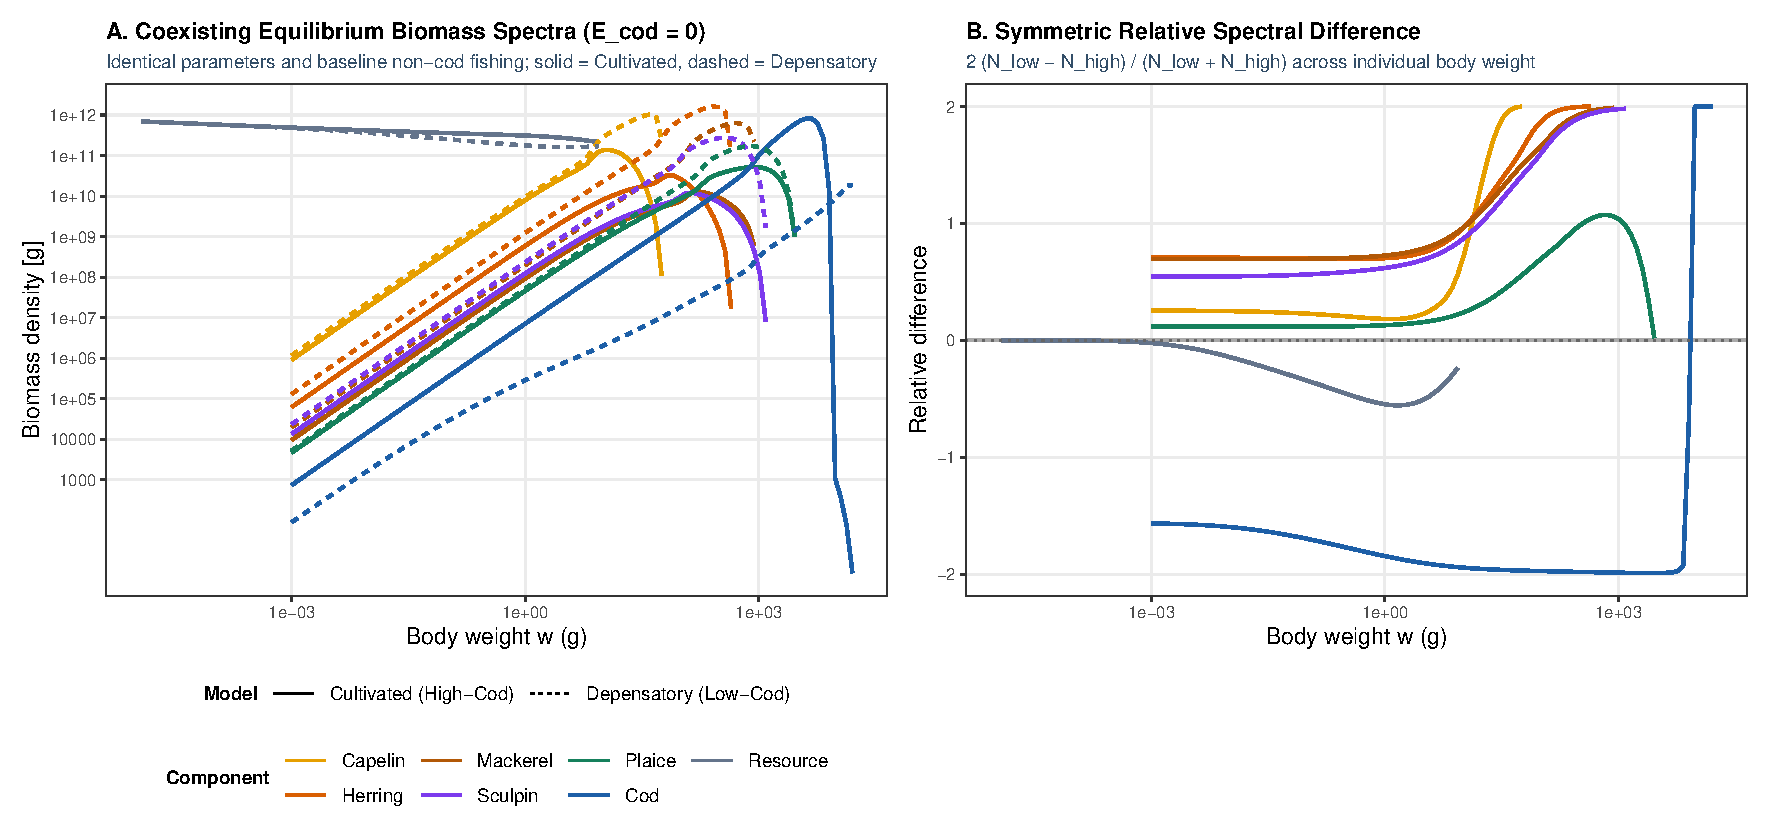
\includegraphics[width=0.98\textwidth]{figures/fig2_size_spectra_cascade.pdf}
  \caption{Coexisting zero-cod-fishing ($E_{\mathrm{cod}} = 0\text{ yr}^{-1}$) community size spectra under identical model parameters (baseline non-cod fleets active). \textbf{(A)} Biomass density per unit log body mass, $w^2 N(w)$, across resource and consumer guilds. \textbf{(B)} Symmetric relative difference $2(N_{\mathrm{low}} - N_{\mathrm{high}})/(N_{\mathrm{low}} + N_{\mathrm{high}}) \in [-2, 2]$, showing resource grazing below $10\text{ g}$, $5$--$900\text{ g}$ forage/sculpin expansion, truncation of $0.05$--$8\text{ kg}$ cod, and survival of ultra-trace $>8\text{ kg}$ low-state cod to larger asymptotic mass ($15\text{ kg}$) than food-limited cultivated adults ($\sim 9.5\text{ kg}$).}
  \label{fig:spectra}
\end{figure}

Crucially, basin boundaries in this 727-dimensional system cannot be reduced to a universal scalar cod-SSB threshold. Along the straight state-space chord $(1 - \alpha)(N_{\mathrm{low}}, N_{R,\mathrm{low}}) + \alpha(N_{\mathrm{high}}, N_{R,\mathrm{high}})$ verified for monotonicity over a $1000\text{ yr}$ horizon, the transition bracket lies at $\mathrm{SSB}_{\mathrm{cod}} \in [28.42, 28.48]\text{ kt}$ for $E_{\mathrm{cod}} = 0$ and $[242.49, 242.54]\text{ kt}$ for $E_{\mathrm{cod}} = 0.15\text{ yr}^{-1}$ (using the true $E_{\mathrm{cod}} = 0.15$ low endpoint), whereas the Newton-polished unstable saddle fixed points have cod SSBs of $42.1\text{ kt}$ ($E_{\mathrm{cod}} = 0$, $n_+ = 1$, $\lambda_+ = +0.00813\text{ yr}^{-1}$) and $321.7\text{ kt}$ ($E_{\mathrm{cod}} = 0.15\text{ yr}^{-1}$, $n_+ = 1$, $\lambda_+ = +0.07781\text{ yr}^{-1}$; Table~\ref{tab:equilibria}). Constructing states with identical or inverted cod SSB but contrasting prey communities proves path dependence directly: at $E_{\mathrm{cod}} = 0$, $22.0\text{ kt}$ cod SSB paired with the cultivated prey spectrum ($315.1\text{ kt}$ forage, $27.3\text{ kt}$ sculpin) converges to $1018.2\text{ kt}$, whereas both $22.0\text{ kt}$ and $35.0\text{ kt}$ cod SSB ($> 28.5\text{ kt}$ chord bracket) paired with the depensatory prey spectrum ($4976.3\text{ kt}$ forage, $548.3\text{ kt}$ sculpin) collapse to $15.8\text{ kt}$. Similarly, at $E_{\mathrm{cod}} = 0.15\text{ yr}^{-1}$, $180.0\text{ kt}$ cod SSB converges to $776.3\text{ kt}$ in cultivated prey but collapses to $1.29\text{ kt}$ in depensatory prey.

\subsection{Predator-Resolved Mortality, Ontogenetic Feeding Shifts, and $R_0$ Decomposition}

Decomposing vital rates across body size clarifies both the early-life bottleneck and its opposing adult bioenergetic response (Fig.~\ref{fig:mechanisms}). Across the $0.05$--$5\text{ g}$ nursery window, unweighted bin-mean cod predation mortality rises from $0.25\text{ yr}^{-1}$ (cultivated $E_{\mathrm{cod}} = 0$) and $0.69\text{ yr}^{-1}$ ($E_{\mathrm{cod}} = 0.15$) to $7.33\text{ yr}^{-1}$ (depensatory $E_{\mathrm{cod}} = 0$), closely matching abundance-weighted cohort means ($0.22$, $0.63$, and $7.39\text{ yr}^{-1}$). Because instantaneous mortality ratios do not equal survival ratios, we integrate the cumulative hazard $H = \int (\mu/g)\,\mathrm{d}w$ directly (eq.~\ref{eq:survival}; Fig.~\ref{fig:mechanisms}C). Across $[0.001, 15)\text{ g}$, $H$ increases from $0.185$ in the cultivated state to $2.821$ in the depensatory state ($\Delta H = +2.636$), reducing stationary cohort survival $14.0$-fold from $83.1\%$ to $6.0\%$ (discrete upwind product $83.1\%$ to $6.6\%$, $12.6$-fold; across all pre-maturation sizes $[0.001, 850)\text{ g}$, $H$ rises from $0.623$ to $3.815$, cutting survival $24.3$-fold from $53.6\%$ to $2.2\%$).

\begin{figure}[t!]
  \centering
  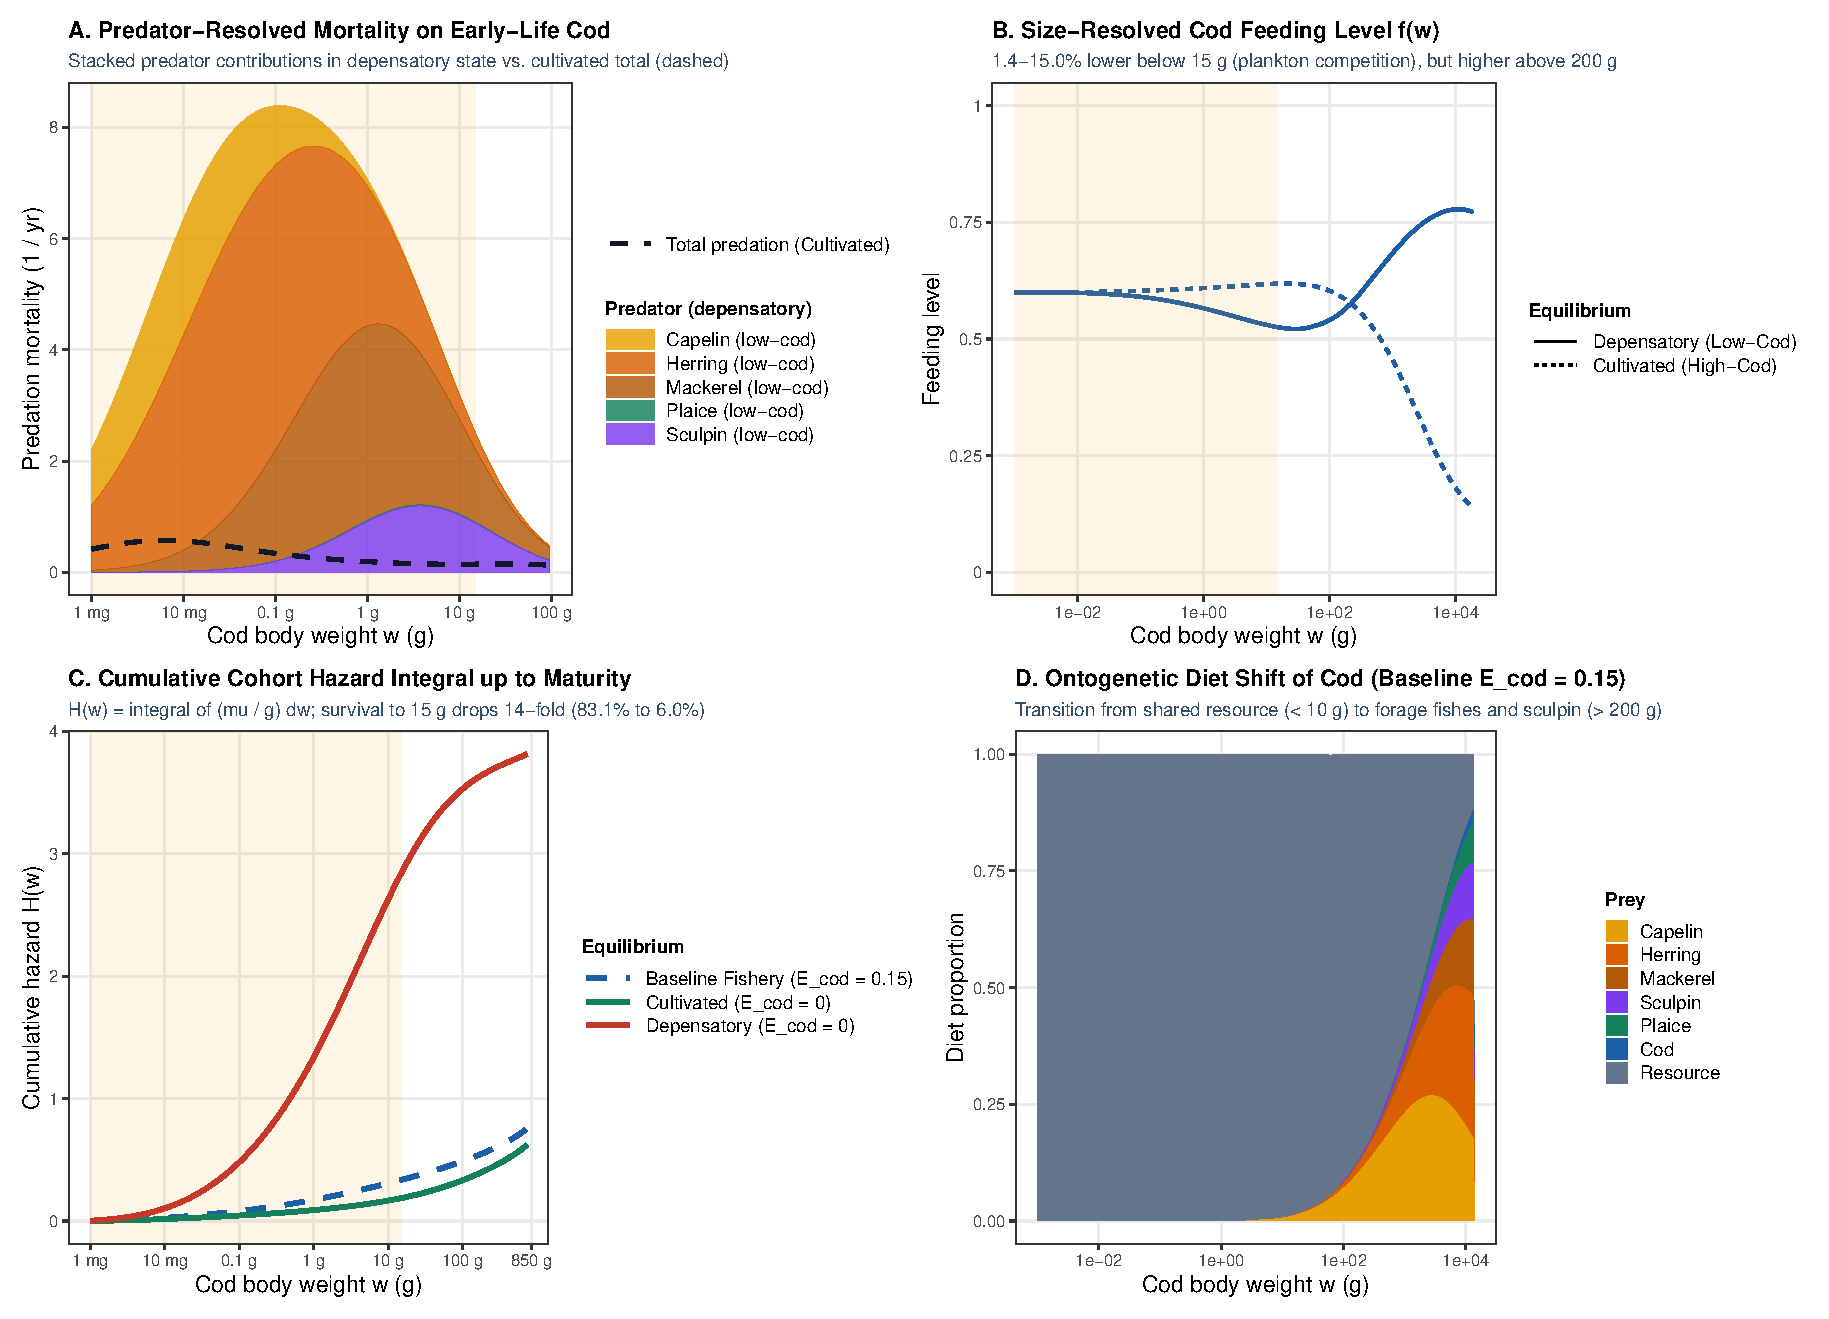
\includegraphics[width=0.96\textwidth]{figures/fig3_trophic_mechanisms.pdf}
  \caption{Predator-resolved demographic bottleneck and opposing ontogenetic feeding shifts. \textbf{(A)} Instantaneous predation mortality $\mu_p(w)$ on cod decomposed by predator guild in the depensatory state vs.\ total cultivated $\mu_p(w)$ ($E_{\mathrm{cod}} = 0$). \textbf{(B)} Cod feeding level $f(w)$ comparing depensatory vs.\ cultivated $E_{\mathrm{cod}} = 0$ equilibria ($1.4\%$--$15.0\%$ lower below $15\text{ g}$, higher above $200\text{ g}$). \textbf{(C)} Cumulative hazard $H(w) = \int_{w_0}^w (\mu/g)\,\mathrm{d}w'$ from $1\text{ mg}$ to maturation ($850\text{ g}$) across the three reference equilibria. \textbf{(D)} Cod diet proportions by prey guild at the baseline fished equilibrium ($E_{\mathrm{cod}} = 0.15\text{ yr}^{-1}$).}
  \label{fig:mechanisms}
\end{figure}

Exact two-way decomposition of $\Delta H = +2.636$ on $[0.001, 15)\text{ g}$ attributes $+2.339$ ($88.7\%$) to higher mortality evaluated at cultivated growth, $+0.023$ ($0.9\%$) to slower growth alone evaluated at cultivated mortality, and $+0.274$ ($10.4\%$) to the multiplicative interaction between elevated predation and slower growth. Resolving low-state $[0.001, 15)\text{ g}$ hazard by mortality source (Fig.~\ref{fig:mechanisms}A) shows that mackerel ($H = 1.153$), herring ($0.980$), and sculpin ($0.420$) generate $93.8\%$ of total predation hazard ($2.721$), whereas capelin contributes only $0.161$ ($5.9\%$), plaice $0.007$, and background mortality $0.100$.

Shared resource grazing by expanded planktivores lowers cod feeding level $f(w)$ in the depensatory state by $1.35\%$--$11.68\%$ relative ($-0.81$ to $-7.17$ percentage points; low/high ratio $0.883$--$0.987$) across $0.05$--$5\text{ g}$, and by $0.07\%$--$15.00\%$ relative ($-0.04$ to $-9.28$ percentage points; ratio $0.850$--$0.999$) across $0.002$--$15\text{ g}$ (Fig.~\ref{fig:mechanisms}B). Above $200\text{ g}$, however, cod transition onto fish prey (Fig.~\ref{fig:mechanisms}D), so rare surviving $1$--$10\text{ kg}$ cod experience $52\%$--$321\%$ \emph{higher} feeding levels ($+23.6$ to $+59.3$ percentage points) in the depensatory state than in the food-limited cultivated state (explaining the $>8\text{ kg}$ tail in Fig.~\ref{fig:spectra}B). A six-way factorial over $(\mu, g, e_r)$ shows how juvenile mortality overwhelms this adult fecundity boost: cod net reproductive ratio $R_0(\mu_{\mathrm{high}}, g_{\mathrm{high}}, e_{r,\mathrm{high}}) = 1.21$ drops to $0.57$ under low-state growth alone $(\mu_{\mathrm{high}}, g_{\mathrm{low}}, e_{r,\mathrm{high}})$, plunges to $0.086$ under low-state mortality $(\mu_{\mathrm{low}}, g_{\mathrm{high}}, e_{r,\mathrm{high}})$ and $0.027$ under combined $(\mu_{\mathrm{low}}, g_{\mathrm{low}}, e_{r,\mathrm{high}})$, and recovers only to $R_0(\mu_{\mathrm{low}}, g_{\mathrm{low}}, e_{r,\mathrm{low}}) = 0.883 < 1$ once elevated adult reproductive output $e_{r,\mathrm{low}}$ is included ($1/(1 - R_0) = 8.53$, matching the $13.5\%$ exogenous share of low-state recruitment up to Beverton--Holt saturation). Counterfactual projections from \texttt{cod\_low\_f0} confirm that either zeroing non-cod predation on cod ($\theta_{i,\mathrm{Cod}} = 0$ for $i \neq \mathrm{Cod}$) or clamping $N_R(w)$ at cultivated resource levels triggers escape to $> 1018\text{ kt}$ cod SSB, though clamping $N_R(w)$ simultaneously alters predator intake $1 - f_i(w)$ in eq.~\eqref{eq:predmort}.

\subsection{Hysteresis Continuation, Transition Intervals, and Escape Timescales}

Fallback-free continuation scans paired with fine $0.005\text{ yr}^{-1}$ settled refinements (\texttt{project} settling plus \texttt{newton} polish) bracket both hysteresis transitions cleanly (Fig.~\ref{fig:hysteresis}). Along the upper cod-fishing branch, equilibrium cod SSB declines smoothly from $1018.2\text{ kt}$ ($E_{\mathrm{cod}} = 0$) to $580.5\text{ kt}$ at $E_{\mathrm{cod}} = 0.240\text{ yr}^{-1}$ while the leading real eigenvalue approaches zero monotonically ($\max\operatorname{Re}(\lambda) = -0.166\text{ yr}^{-1}$ at $0.215$, $-0.119$ at $0.230$, and $-0.0435\text{ yr}^{-1}$ at $0.240\text{ yr}^{-1}$), before dropping across $E_{\mathrm{cod}} \in [0.240, 0.245]\text{ yr}^{-1}$ to $0.75\text{ kt}$ on the lower branch (Fig.~\ref{fig:hysteresis}A). Decreasing $E_{\mathrm{cod}}$ from $0.50$ back to $0.00\text{ yr}^{-1}$ tracks the lower branch continuously to $15.8\text{ kt}$.

\begin{figure}[t!]
  \centering
  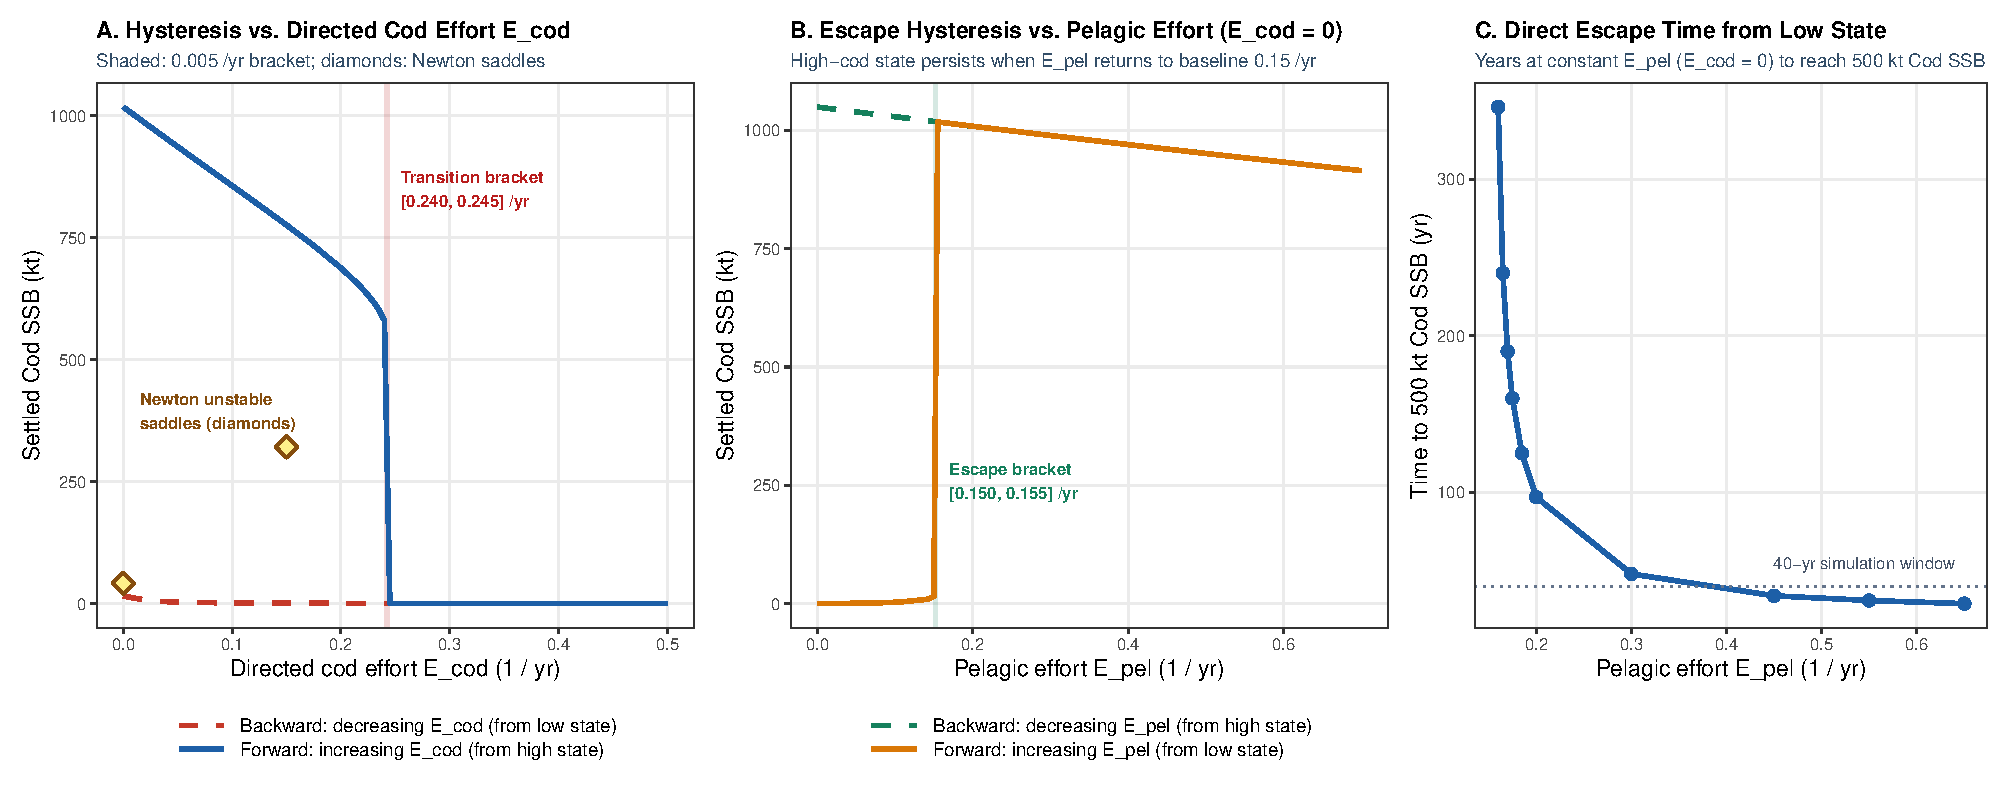
\includegraphics[width=0.98\textwidth]{figures/fig4_hysteresis_bifurcation.pdf}
  \caption{Hysteresis continuation curves, Newton-polished unstable saddles (diamonds), and escape timescales. \textbf{(A)} Settled cod SSB vs.\ directed cod effort $E_{\mathrm{cod}}$ ($E_{\mathrm{pel}} = 0.15\text{ yr}^{-1}$), transitioning across $[0.240, 0.245]\text{ yr}^{-1}$. \textbf{(B)} Settled cod SSB vs.\ 4-gear pelagic effort $E_{\mathrm{pel}}$ at $E_{\mathrm{cod}} = 0$, escaping across $[0.150, 0.155]\text{ yr}^{-1}$ over multi-century horizons. \textbf{(C)} Direct escape time from \texttt{cod\_low\_f0} to $500\text{ kt}$ cod SSB at constant $E_{\mathrm{pel}}$ ($E_{\mathrm{cod}} = 0$) relative to a 40-year window.}
  \label{fig:hysteresis}
\end{figure}

Scanning 4-gear pelagic effort $E_{\mathrm{pel}}$ upward from \texttt{cod\_low\_f0} at $E_{\mathrm{cod}} = 0$ locates the asymptotic escape transition within $E_{\mathrm{pel}} \in [0.150, 0.155]\text{ yr}^{-1}$ ($\mathrm{SSB}_{\mathrm{cod}} = 15.8\text{ kt}$ at $0.150\text{ yr}^{-1}$ vs.\ $1017.2\text{ kt}$ after $927\text{ yr}$ at $0.155\text{ yr}^{-1}$; Fig.~\ref{fig:hysteresis}B). Proximity of baseline pelagic fishing ($0.150\text{ yr}^{-1}$) to this transition explains the weak $-0.0084\text{ yr}^{-1}$ eigenvalue at \texttt{cod\_low\_f0} and produces severe multi-century transients just above the threshold (Fig.~\ref{fig:hysteresis}C): directly simulated time from \texttt{cod\_low\_f0} to reach $500\text{ kt}$ cod SSB falls from $346\text{ yr}$ ($E_{\mathrm{pel}} = 0.160$) and $160\text{ yr}$ ($0.175$) to $97\text{ yr}$ ($0.200$), $48\text{ yr}$ ($0.300$), $34\text{ yr}$ ($0.450$), and $29\text{ yr}$ ($0.650\text{ yr}^{-1}$).

\subsection{Matched Six-Gear Policies, Capelin Sparing, Bycatch Limits, and Feedback Control}

Evaluating post-closure interventions from $t = 61\text{ yr}$ ($\tau \in [0, 40]\text{ yr}$, verified to $\tau = 340\text{ yr}$; Table~\ref{tab:policies}; Figs.~\ref{fig:scenarios}--\ref{fig:surface}) separates transient $\tau = 40\text{ yr}$ states from asymptotic outcomes and isolates each policy mechanism:
\begin{enumerate}
  \item \textbf{Closure, premature reopening, and single-guild harvest:} Status-quo closure (\#1; Fig.~\ref{fig:scenarios}A) reaches $11.4\text{ kt}$ cod SSB at $\tau = 40\text{ yr}$ ($15.5\text{ kt}$ at $\tau = 340\text{ yr}$), whereas unassisted cod reopening at $E_{\mathrm{cod}} = 0.25\text{ yr}^{-1}$ (\#2) depresses cod to $0.7\text{ kt}$. Sustained sculpin-only harvest ($E_{\mathrm{meso}} = 0.45\text{ yr}^{-1}$, \#3) reaches only $32.1\text{ kt}$ by $\tau = 40\text{ yr}$ yet eventually escapes over multi-century timescales ($1013.2\text{ kt}$ at $\tau = 340\text{ yr}$; Fig.~\ref{fig:scenarios}C), whereas sustained pelagic harvest ($E_{\mathrm{pel}} = 0.55\text{ yr}^{-1}$, \#4) rebuilds cod to $937.8\text{ kt}$ by $\tau = 40\text{ yr}$ ($941.5\text{ kt}$ asymptotically).
  \item \textbf{Matched test of tapering vs.\ sustained thinning at $E_{\mathrm{cod}} = 0.15\text{ yr}^{-1}$:} Holding Phase-I efforts ($0.65, 0.45\text{ yr}^{-1}$) and Phase-II cod reopening ($E_{\mathrm{cod}} = 0.15\text{ yr}^{-1}$ at $\tau = 20\text{ yr}$) identical, cod SSB at the $\tau = 20\text{ yr}$ switch is $248.6\text{ kt}$---not yet rebuilt, and barely above the $242.5\text{ kt}$ chord bracket. Sustaining heavy forage/sculpin harvest (\#6) reaches $658.5\text{ kt}$ at $\tau = 40\text{ yr}$ ($665.3\text{ kt}$ asymptotically; $40\,179\text{ kt}$ 40-yr cumulative catch), whereas tapering back to baseline at $\tau = 20\text{ yr}$ (\#7; Fig.~\ref{fig:scenarios}C) slows mid-term cod rebuilding ($433.6\text{ kt}$ at $\tau = 40\text{ yr}$; $35\,425\text{ kt}$ cumulative catch) in exchange for restoring the higher $776.3\text{ kt}$ cultivated cod equilibrium and avoiding chronic pelagic depletion. Across all 42 Phase-I $(E_{\mathrm{pel}}, E_{\mathrm{meso}})$ grid cells under this fixed 20-year taper with $E_{\mathrm{cod}} = 0.15\text{ yr}^{-1}$, only five cells recover asymptotically (asterisks in Fig.~\ref{fig:surface}A); notably, $(0.65, 0.35)$ reaches $263\text{ kt}$ at $\tau = 40\text{ yr}$ ($> 242.5\text{ kt}$ chord bracket) yet still collapses asymptotically to $1.3\text{ kt}$.
  \item \textbf{Capelin sparing vs.\ joint pelagic fishing:} Unexploited ($E_{\mathrm{cap}} = 0$) capelin cutoff-biomass benchmarks are $B_{0,\mathrm{Cap}}^{\mathrm{high}} = 234.7\text{ kt}$ in the zero-cod-fishing cultivated state and $B_{0,\mathrm{Cap}}^{f15} = 382.3\text{ kt}$ at $E_{\mathrm{cod}} = 0.15\text{ yr}^{-1}$. Because herring, mackerel, and sculpin---not capelin---dominate $<15\text{ g}$ cod hazard, keeping \texttt{Capelin\_Gear} at baseline ($E_{\mathrm{cap}} = 0.15\text{ yr}^{-1}$, \#8; Fig.~\ref{fig:scenarios}B) or zero ($E_{\mathrm{cap}} = 0$, \#9) while harvesting herring/mackerel ($0.65\text{ yr}^{-1}$) and sculpin ($0.45\text{ yr}^{-1}$) \emph{accelerates} cod rebuilding ($344.7\text{ kt}$ at $\tau = 20\text{ yr}$ and $745.8\text{ kt}$ at $\tau = 40\text{ yr}$ in \#8 vs.\ $248.6$ and $433.6\text{ kt}$ in \#7) while keeping minimum Phase-I capelin cutoff biomass at $1327.0\text{ kt}$ (vs.\ $793.0\text{ kt}$ under joint pelagic fishing).
  \item \textbf{Multi-objective yield trade-offs (no monetary valuation):} Table~\ref{tab:policies} and Fig.~\ref{fig:surface}B,C distinguish 40-year cumulative catch, $\tau = 40\text{ yr}$ transient annual yield, and asymptotic equilibrium yield. Rebuilding the cultivated cod fishery ($191.9\text{ kt}\cdot\text{yr}^{-1}$ asymptotic total yield in \#7--\#9, including $128.5\text{ kt}\cdot\text{yr}^{-1}$ cod) delivers \emph{lower} equilibrium aggregate tonnage than continuously harvesting hyperabundant planktivores in the status-quo depensatory state ($660.7\text{ kt}\cdot\text{yr}^{-1}$ in \#1). Because the model contains no prices or harvesting costs, choosing between high-volume forage landings and gadoid rebuilding is a normative conservation and fleet-composition trade-off, not an aggregate biomass-yield gain.
  \item \textbf{Phase-I cod bycatch fragility vs.\ noisy feedback HCR:} Adding incidental cod effort during Phase~I ($\tau \in [0, 20)\text{ yr}$) reveals extreme fragility of the fixed 20-year joint pulse (\#7; Fig.~\ref{fig:scenarios}D): recovery succeeds at $E_{\mathrm{byc}} \le 0.005\text{ yr}^{-1}$ ($776.3\text{ kt}$ asymptotically) but fails asymptotically at $E_{\mathrm{byc}} \ge 0.010\text{ yr}^{-1}$ for both juvenile and adult selectivity (reverting to $1.29\text{ kt}$ at $\tau = 340\text{ yr}$ despite deceptive transient $\tau = 40\text{ yr}$ cod SSBs of $270.7$ and $306.4\text{ kt}$; Table~\ref{tab:policies}). Capelin sparing (\#8) widens bycatch tolerance four- to six-fold ($E_{\mathrm{byc}} \le 0.020\text{ yr}^{-1}$ juvenile; $\le 0.030\text{ yr}^{-1}$ adult). Replacing the fixed $\tau = 20\text{ yr}$ calendar switch with the lagged state-dependent feedback HCR ($\widehat{\mathrm{SSB}}_{\mathrm{cod}} \ge 280\text{ kt}$ for two consecutive years, $\mathrm{CV} = 0.25$ lognormal observation error; Fig.~\ref{fig:scenarios}C) switches between $\tau = 21$ and $25\text{ yr}$ (median $23.0\text{ yr}$) and achieves $100\%$ ($16/16$) asymptotic recovery ($765.1\text{ kt}$ mean $\tau = 40\text{ yr}$ SSB; Table~\ref{tab:policies}).
\end{enumerate}

\begin{figure}[t!]
  \centering
  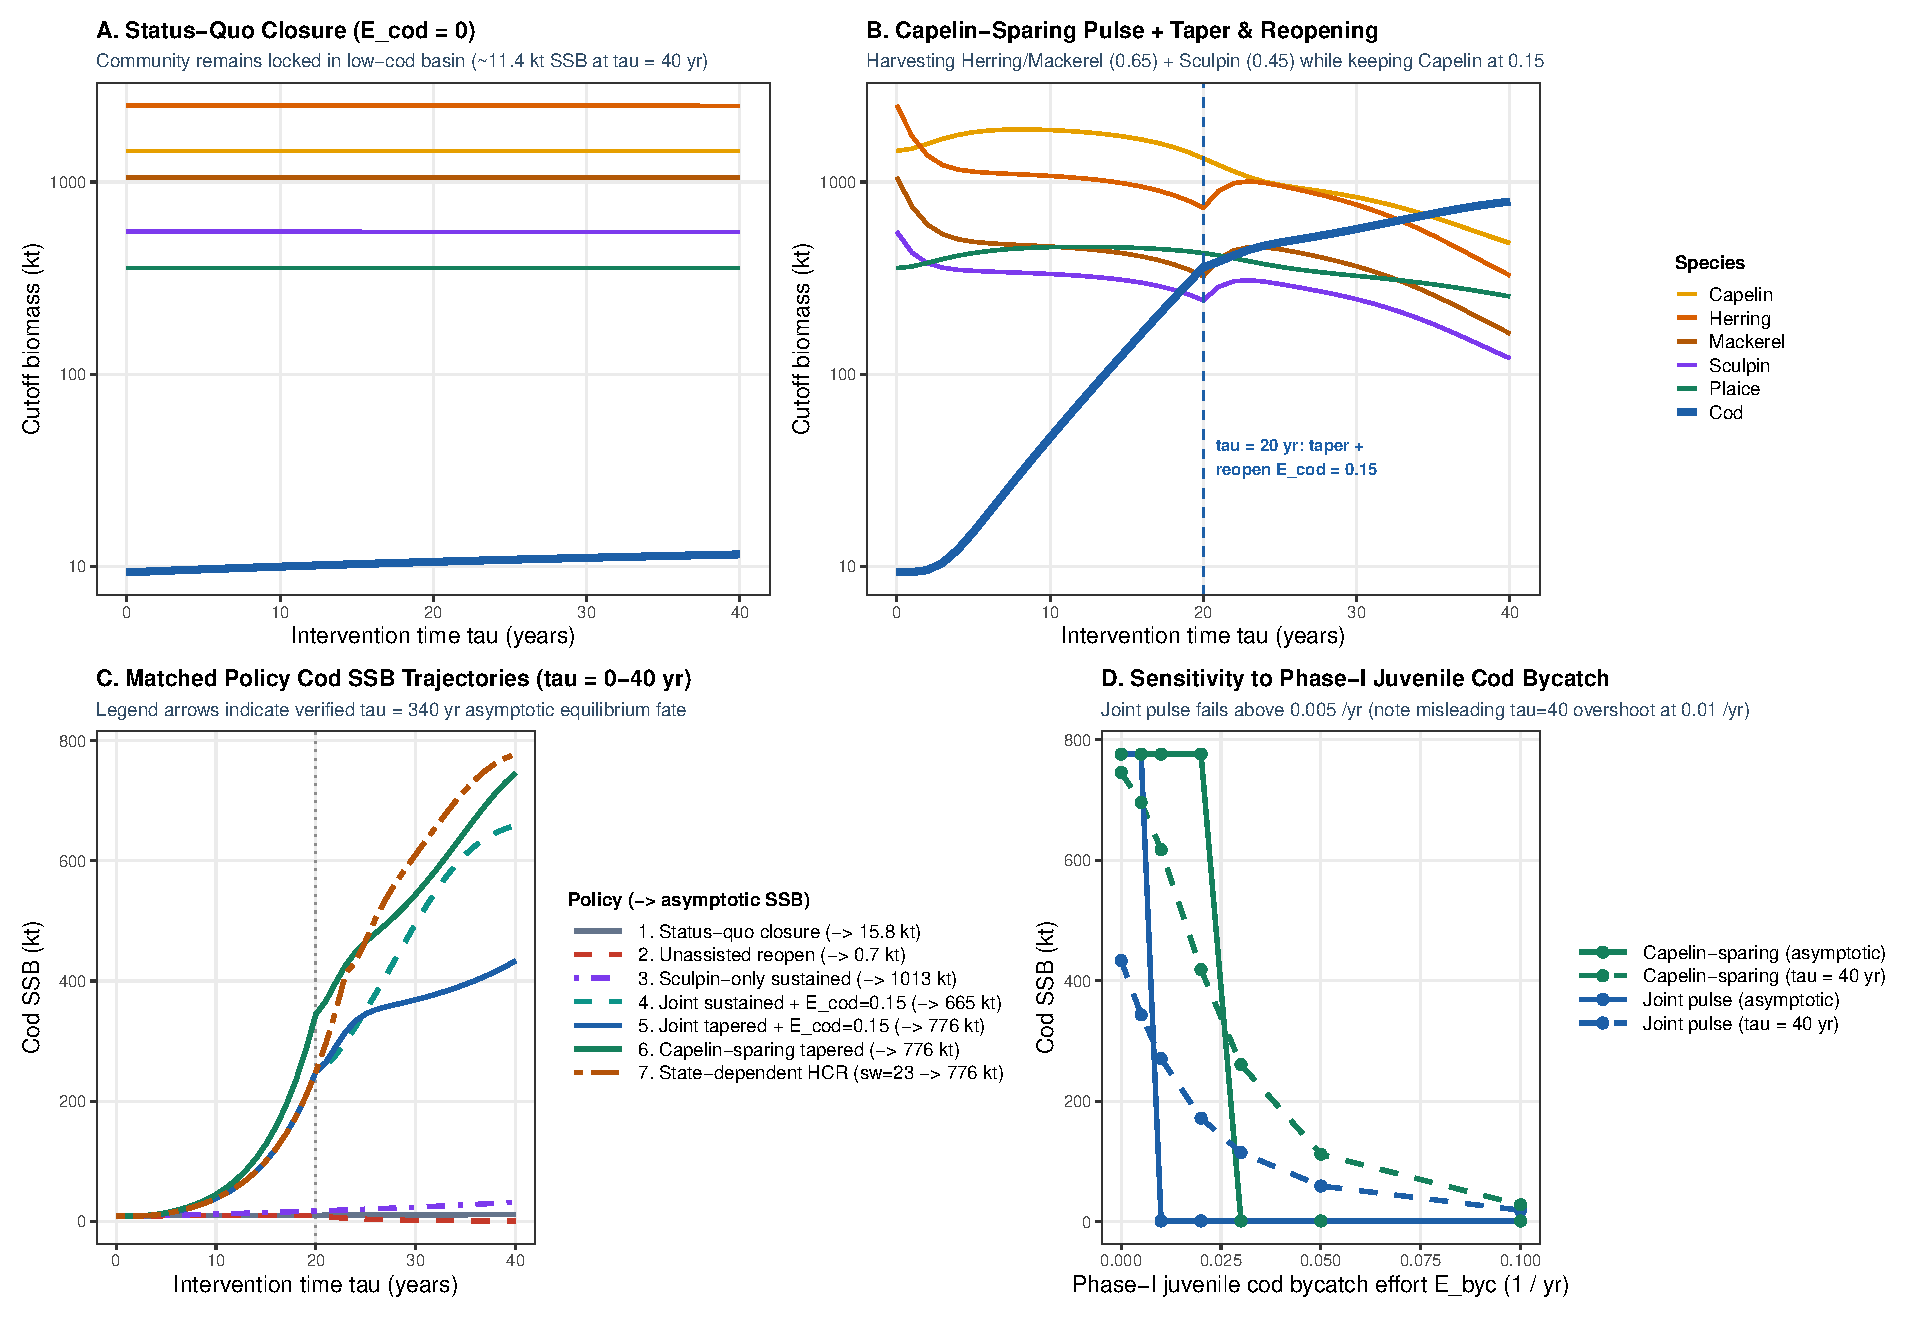
\includegraphics[width=0.95\textwidth]{figures/fig5_recovery_strategies.pdf}
  \caption{Post-closure 6-gear ecosystem trajectories and bycatch sensitivity ($\tau = 0$--$40\text{ yr}$ from $t = 61\text{ yr}$; \texttt{tr\_bdf2}, $\Delta t = 0.05\text{ yr}$; panels A and B plot cutoff biomasses $w \ge w_{\mathrm{cut},i}$). \textbf{(A)} Status-quo closure (\#1). \textbf{(B)} Capelin-sparing pulse with $\tau = 20\text{ yr}$ taper and reopened $E_{\mathrm{cod}} = 0.15\text{ yr}^{-1}$ (\#8). \textbf{(C)} Cod SSB across seven matched policies (legend arrows report verified $\tau = 340\text{ yr}$ asymptotic fates). \textbf{(D)} Sensitivity of $\tau = 40\text{ yr}$ (dashed) vs.\ asymptotic $\tau = 340\text{ yr}$ (solid) cod SSB to Phase-I juvenile cod bycatch $E_{\mathrm{byc,juv}}$, contrasting the joint pulse (\#7) against capelin sparing (\#8).}
  \label{fig:scenarios}
\end{figure}

\begin{table}[t!]
\centering
\caption{Matched 6-gear post-closure policy experiments initialized from $t = 61\text{ yr}$ ($\mathrm{SSB}_{\mathrm{cod}} = 9.17\text{ kt}$; $E_{\mathrm{flat}} = 0.15\text{ yr}^{-1}$ throughout). Tuples list $(E_{\mathrm{cap}}, E_{\mathrm{hm}}, E_{\mathrm{meso}})$ in $\text{yr}^{-1}$, with $\mathrm{B} = (0.15, 0.15, 0.05)$; arrows ($\to$) mark $\tau = 20\text{ yr}$ transitions and $|E_{\mathrm{cod}}$ gives Phase-II cod effort ($0$ in Phase~I unless bycatch is noted). Asymptotic SSB and annual yield ($\text{kt}\cdot\text{yr}^{-1}$) are evaluated at $\tau = 340\text{ yr}$.}
\label{tab:policies}
\vspace{0.3em}
{\footnotesize
\setlength{\tabcolsep}{1.9pt}
\begin{tabular}{@{}llrrrrrrrc@{}}
\toprule
Strategy & Ph-I $\to$ II Schedule & $\tau=20$ & $\tau=40$ & Asymp. & Min Cap. & Cum.\ Yld & $\tau=40$ & Asymp. & Recov. \\
         & $(E_{\mathrm{cap}}, E_{\mathrm{hm}}, E_{\mathrm{meso}}) \mid E_{\mathrm{cod}}$ & SSB & SSB & SSB & (kt) & (kt) & Yld & Yld & Basin? \\
\midrule
1. Closure           & $\mathrm{B} \mid 0.00$                       &  10.4 &  11.4 &   15.5 & 1451.6 & 26\,574 & 663.6 & 660.7 & No \\
2. Reopen $0.25$     & $\mathrm{B} \mid 0.25$                       &  10.4 &   0.9 &    0.7 & 1451.6 & 26\,688 & 671.1 & 671.2 & No \\
3. Sculpin only      & $(0.15,0.15,0.45) \mid 0.00$                 &  17.5 &  32.1 & 1013.2 & 1451.7 & 30\,816 & 759.2 &  43.2 & Yes$^{\mathrm{a}}$ \\
4. Pelagic ($f_0$)   & $(0.55,0.55,0.05) \mid 0.00$                 &  85.5 & 937.8 &  941.5 &  917.4 & 38\,715 & 176.1 &  94.2 & Yes \\
5. Sustain ($f_0$)   & $(0.65,0.65,0.45) \mid 0.00$                 & 248.6 & 933.6 &  918.5 &  793.0 & 34\,589 & 106.2 & 111.9 & Yes \\
6. Sustain ($f_{15}$)& $(0.65,0.65,0.45) \mid 0.15$                 & 248.6 & 658.5 &  665.3 &  793.0 & 40\,179 & 368.0 & 342.4 & Yes \\
7. Taper ($f_{15}$)  & $(0.65,0.65,0.45)\!\to\!\mathrm{B}\mid 0.15$ & 248.6 & 433.6 &  776.3 &  793.0 & 35\,425 & 391.3 & 191.9 & Yes \\
8. Spare cap.\ (base)& $(0.15,0.65,0.45)\!\to\!\mathrm{B}\mid 0.15$ & 344.7 & 745.8 &  776.3 & 1327.0 & 29\,105 & 229.5 & 191.9 & Yes \\
9. Spare cap.\ (zero)& $(0.00,0.65,0.45)\!\to\!\mathrm{B}\mid 0.15$ & 377.2 & 767.9 &  776.3 & 1451.7 & 25\,450 & 216.4 & 191.9 & Yes \\
\midrule
7b. $\#7+$byc.\ $0.01$ & $\#7 + E_{\mathrm{byc,juv}}=0.010$         & 214.1 & 270.7 &    1.3 &  793.0 & 35\,211 & 474.6 & 670.5 & No \\
8b. $\#8+$byc.\ $0.02$ & $\#8 + E_{\mathrm{byc,juv}}=0.020$         & 256.4 & 418.6 &  776.3 & 1327.0 & 29\,076 & 400.2 & 191.9 & Yes \\
10. Feedback HCR     & $\#7\text{ Ph-I, }2\text{y }\widehat{\mathrm{SSB}}\ge 280$ & ---$^{\mathrm{b}}$ & 765.1 & 776.3 & 793.0 & 34\,889 & 200.4 & 191.9 & 16/16 \\
\bottomrule
\end{tabular}
\par\vspace{0.25em}
{\scriptsize $^{\mathrm{a}}$Multi-century escape ($32.1\text{ kt}$ at $\tau = 40\text{ yr}$). $^{\mathrm{b}}$Median switch $\tau = 23.0\text{ yr}$ ($21$--$25\text{ yr}$ across $16$ noisy $\mathrm{CV}=0.25$ runs, $1\text{ yr}$ lag).}
}
\end{table}

\begin{figure}[t!]
  \centering
  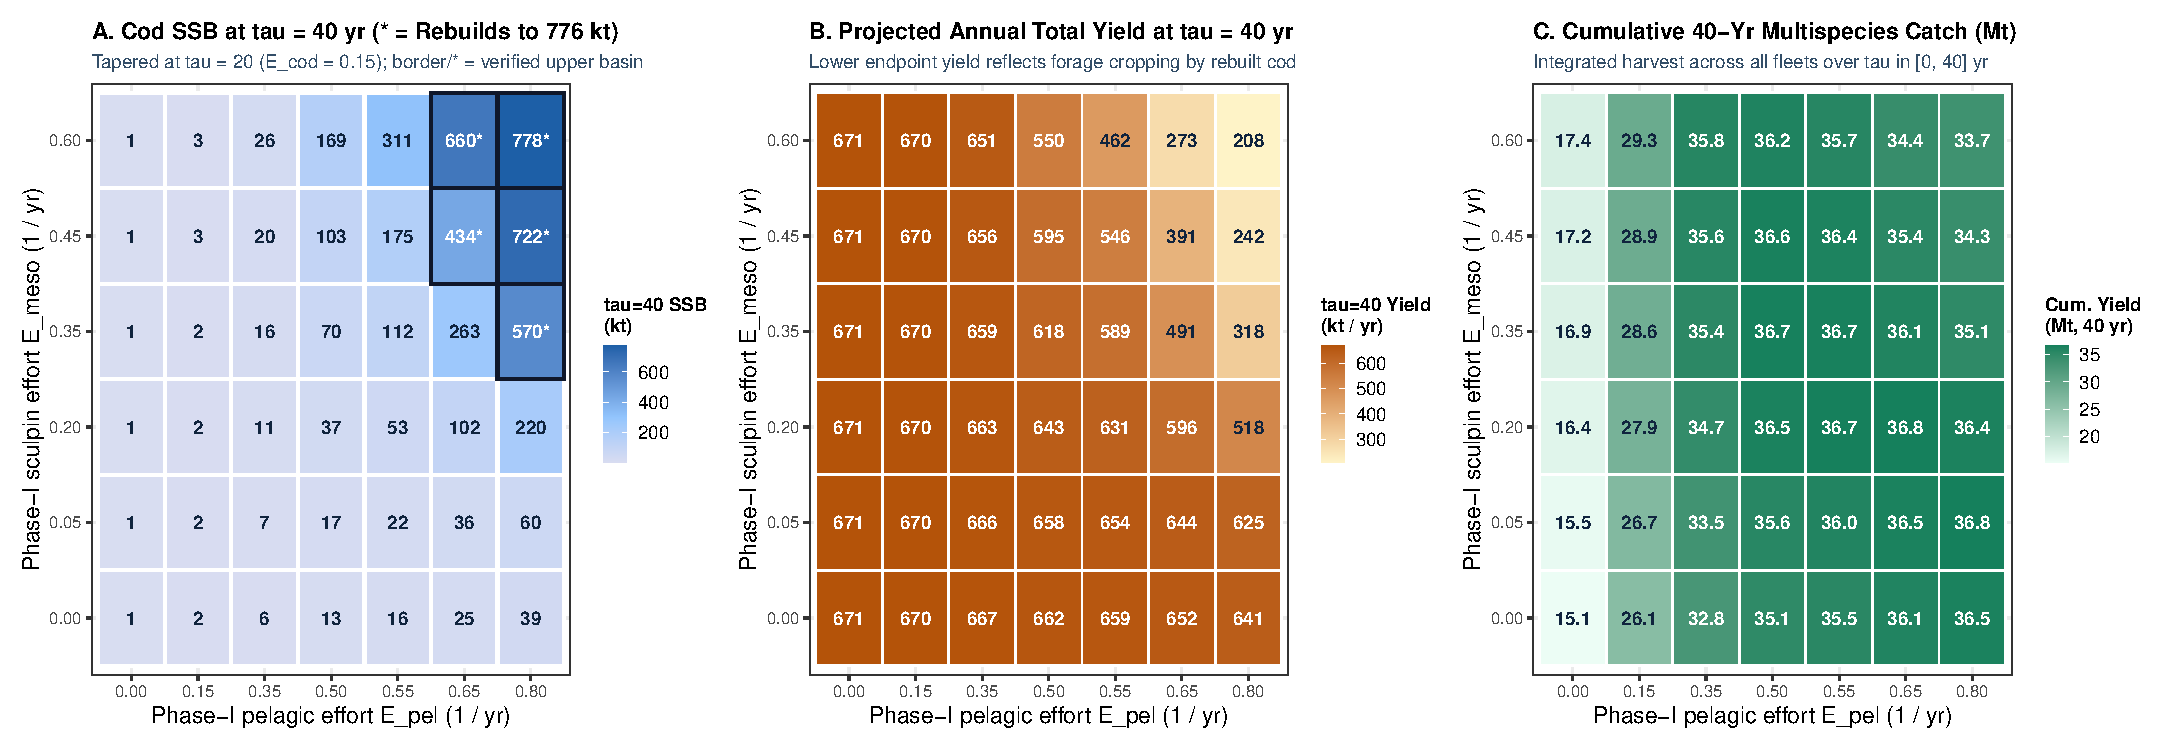
\includegraphics[width=0.98\textwidth]{figures/fig6_policy_tradeoffs.pdf}
  \caption{Two-dimensional 4-gear policy response surface across Phase-I ($\tau \in [0, 20)\text{ yr}$) pelagic effort $E_{\mathrm{pel}}$ and sculpin effort $E_{\mathrm{meso}}$, followed at $\tau = 20\text{ yr}$ by tapering to $(0.15, 0.05)\text{ yr}^{-1}$ and reopening $E_{\mathrm{cod}} = 0.15\text{ yr}^{-1}$. \textbf{(A)} Cod SSB at $\tau = 40\text{ yr}$ (kt); white asterisks (\texttt{*}) mark the only five cells verified to reach the $776.3\text{ kt}$ upper attractor at $\tau = 340\text{ yr}$. \textbf{(B)} Projected annual multispecies yield at $\tau = 40\text{ yr}$ ($\text{kt}\cdot\text{yr}^{-1}$). \textbf{(C)} Cumulative 40-year multispecies catch ($\text{Mt}$, integrated across $\tau \in [0, 40]\text{ yr}$).}
  \label{fig:surface}
\end{figure}

\subsection{Numerical Convergence and Structural Sensitivity Boundaries}
\label{sec:sensitivity}

Time-step, integrator, transport-scheme, and size-grid checks (\texttt{R/04\_\allowbreak sensitivity\_\allowbreak and\_audit.R}; Table~\ref{tab:convergence}; Fig.~\ref{fig:sensitivity}A) resolve both numerical reliability and its limits. First, forensic replay on the archived v1 state confirms that v1's $11.1\%$ policy discrepancy ($475.3\text{ kt}$ vs.\ $422.5\text{ kt}$) arose entirely from Forward Euler time-step truncation between $\Delta t = 0.10$ and $0.20\text{ yr}$ (\texttt{t\_save} had zero effect). Under canonical \texttt{tr\_bdf2}, flagship $\tau = 40\text{ yr}$ cod SSB varies by $< 0.05\%$ between $\Delta t = 0.05\text{ yr}$ ($433.60\text{ kt}$) and $\Delta t = 0.025\text{ yr}$ ($433.80\text{ kt}$), and both flagship and near-boundary $(0.55, 0.20)$ asymptotic classifications remain invariant across $\Delta t \in [0.025, 0.20]\text{ yr}$ (Table~\ref{tab:convergence}A; Fig.~\ref{fig:sensitivity}A). Second, refining consumer grid resolution from $\texttt{no\_w} = 100$ ($\texttt{n\_active} = 727$) to $150$ ($1089$) and $200$ ($1451$), or recalibrating under second-order \texttt{van\_leer} flux limiting, \emph{preserves} zero-cod-fishing bistability and deepens low-state stability ($\mathrm{SSB}_{\mathrm{low}} = 15.8 \to 10.8 \to 10.4\text{ kt}$; $\max\operatorname{Re}(\lambda) = -0.0084 \to -0.0162 \to -0.0172\text{ yr}^{-1}$), whereas coarse $\texttt{no\_w} = 80$ or un-recalibrated \texttt{van\_leer} erases bistability via numerical diffusion shifts (Table~\ref{tab:convergence}B). Because reduced numerical diffusion at $\texttt{no\_w} = 150$--$200$ and recalibrated \texttt{van\_leer} deepens the juvenile bottleneck, the rigid 20-year fixed pulse falls short of the reopened-fishery saddle on finer grids ($\tau = 40\text{ yr}$ SSB $193.8$--$229.6\text{ kt}$, reverting asymptotically), reinforcing the necessity of state-dependent feedback triggers over fixed calendar durations. (Under \texttt{second\_order\_w}, \texttt{getStability()} in \texttt{mizer 3.4.0.9003} raises a non-finite perturbation error at capelin $w = 56.6\text{ g} > w_\infty$, so second-order attractors are verified dynamically; enabling \texttt{bin\_average = TRUE} without single-species growth recalibration fails to settle cleanly.)

\begin{figure}[t!]
  \centering
  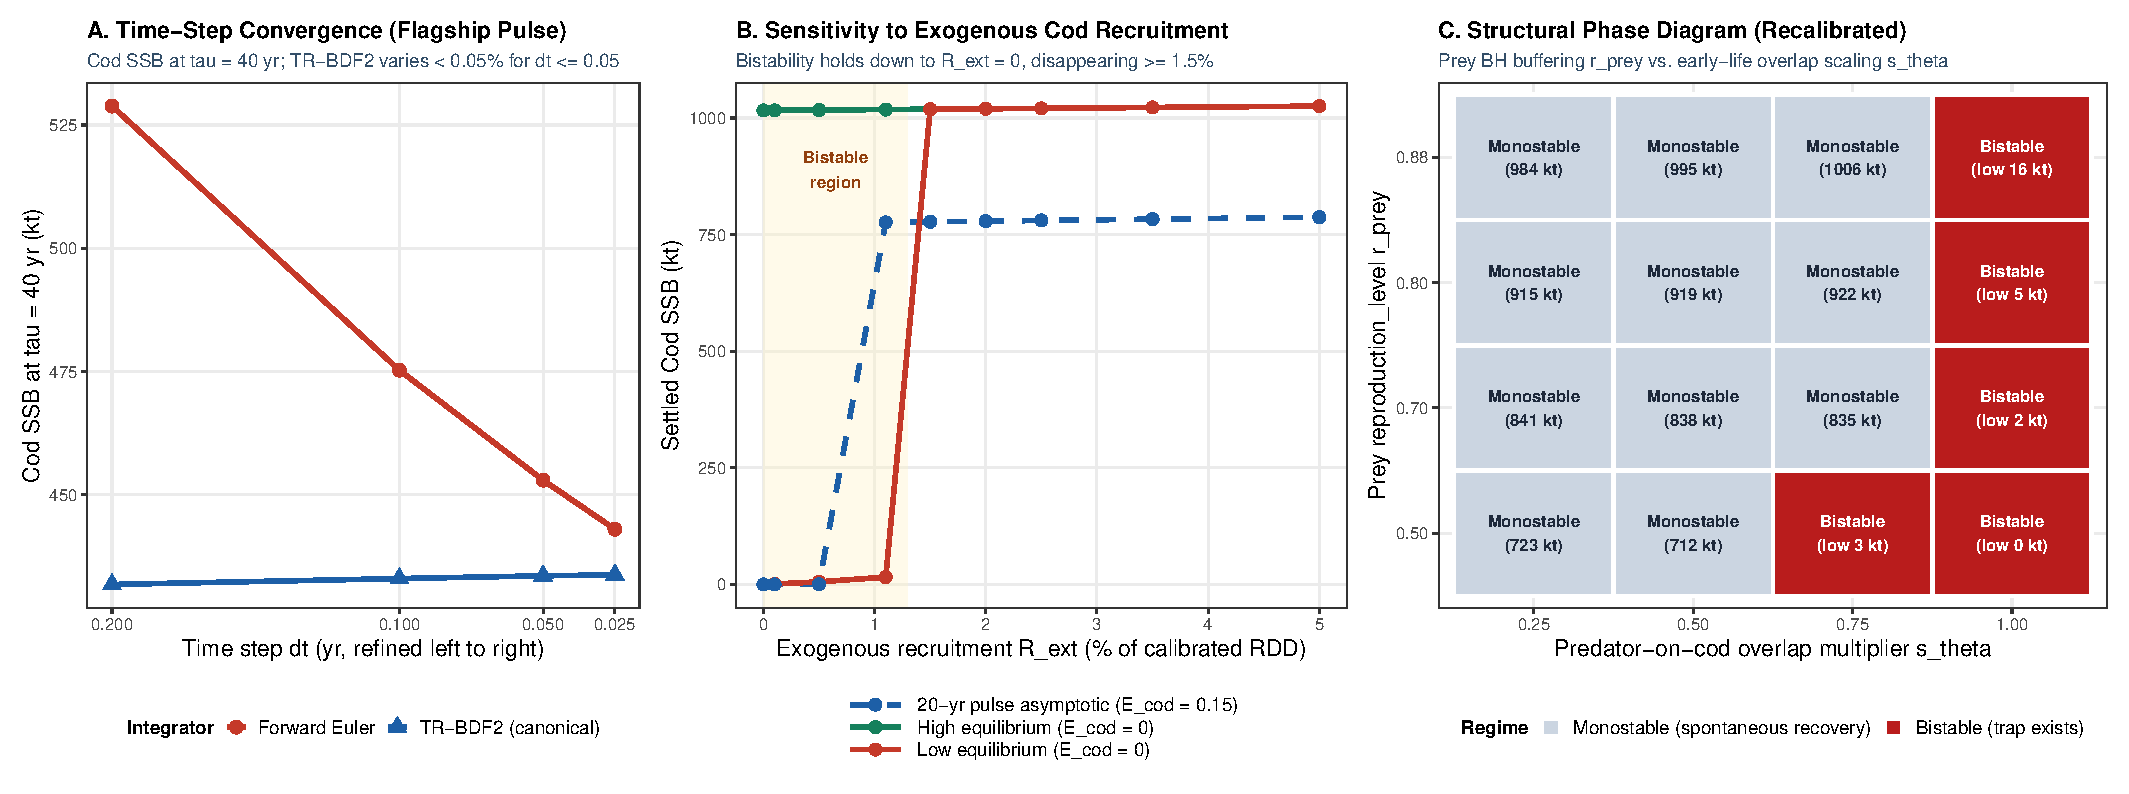
\includegraphics[width=0.99\textwidth]{figures/fig7_structural_sensitivity.pdf}
  \caption{Numerical convergence and structural boundaries of bistability. \textbf{(A)} Time-step convergence of flagship $\tau = 40\text{ yr}$ cod SSB comparing Forward Euler against \texttt{tr\_bdf2}. \textbf{(B)} Settled cod SSB across exogenous cod recruitment $R_{\mathrm{ext,Cod}}$ ($\%$ of calibrated cod recruitment), showing bistability down to $R_{\mathrm{ext,Cod}} = 0$ (where the low state becomes extinction, $R_0 = 0.82 < 1$) and disappearance of the low branch at $\ge 1.5\%$. \textbf{(C)} Recalibrated $4 \times 4$ structural phase diagram across prey Beverton--Holt reproduction level $r_{\mathrm{prey}}$ and predator-on-cod overlap multiplier $s_\theta$ (fixed-parameter perturbations yield the identical $16$-cell regime map).}
  \label{fig:sensitivity}
\end{figure}

\begin{table}[t!]
\centering
\caption{Numerical convergence across time integrators, step sizes $\Delta t$, consumer size-grid resolutions $\texttt{no\_w}$, and spatial advection schemes (\texttt{R/04\_sensitivity\_and\_audit.R}).}
\label{tab:convergence}
\vspace{0.3em}
{\footnotesize
\setlength{\tabcolsep}{3.4pt}
\begin{tabular}{@{}llrrccrc@{}}
\toprule
\multicolumn{8}{@{}l@{}}{\textbf{A. Time-step \& integrator convergence ($\texttt{no\_w} = 100$ upwind; flagship $\#7$ vs.\ $(0.55, 0.20)$)}} \\
\midrule
Integrator & $\Delta t$ (yr) & $t=61$ SSB & Flag.\ $\tau=40$ & Flag.\ Recov. & Near $\tau=40$ & Near Recov. & Bistable? \\
\midrule
Forward Euler          & 0.200 / 0.100          & 11.57 / 10.24          & 528.8 / 475.3          & Yes / Yes          & 69.1 / 59.8 & No / No & Yes \\
Forward Euler          & 0.050 / 0.025          &  9.68 /  9.41          & 453.0 / 443.0          & Yes / Yes          & 56.1 / 54.5 & No / No & Yes \\
\texttt{tr\_bdf2}      & 0.200 / 0.100          &  9.18 /  9.17          & 431.8 / 433.0          & Yes / Yes          & 53.0 / 53.0 & No / No & Yes \\
\texttt{tr\_bdf2} (can.) & \textbf{0.050} / 0.025 & \textbf{9.17} / 9.17 & \textbf{433.6} / 433.8 & \textbf{Yes} / Yes & \textbf{53.0} / 53.0 & \textbf{No} / No & \textbf{Yes} \\
\bottomrule
\end{tabular}

\vspace{0.45em}
\setlength{\tabcolsep}{2.2pt}
\begin{tabular}{@{}lcrrrrrc@{}}
\toprule
\multicolumn{8}{@{}l@{}}{\textbf{B. Consumer size-grid resolution \& advection scheme ($E_{\mathrm{cod}} = 0$ equilibria and 20-yr pulse)}} \\
\midrule
Configuration & Recal.? & $\texttt{no\_w}$ ($N_{\mathrm{act}}$) & High SSB & Low SSB & $\max\operatorname{Re}(\lambda_{\mathrm{low}})$ & Pulse $\tau=40$ & Bist.\ / Recov. \\
\midrule
Upwind ($\texttt{no\_w}=80$)  & Yes      &  80 (581)       & 1003.4         & 1003.4       & $-0.1864$ & 716.0       & No / Yes \\
Upwind ($\texttt{no\_w}=100$) & Yes      & 100 (727)       & 1018.2         &   15.8       & $-0.0084$ & 433.6       & Yes / Yes \\
Upwind ($\texttt{no\_w}=150$) & Yes      & 150 (1089)      & 1023.9         &   10.8       & $-0.0162$ & 229.6       & Yes / No \\
Upwind ($\texttt{no\_w}=200$) & Yes      & 200 (1451)      & 1017.3         &   10.4       & $-0.0172$ & 193.8       & Yes / No \\
\texttt{van\_leer} TVD flux   & No / Yes & 100 (---$^{\mathrm{a}}$) & 938.6 / 1002.9 & 938.6 / 5.5 & ---$^{\mathrm{a}}$ & --- / 65.5 & No / Yes--No \\
\bottomrule
\end{tabular}
\par\vspace{0.25em}
{\scriptsize $^{\mathrm{a}}$In \texttt{mizer 3.4.0.9003}, \texttt{getStability()} errors on \texttt{second\_order\_w} at capelin $w = 56.6\text{ g} > w_\infty$; attractors verified via projection.}
}
\end{table}

\begin{table}[t!]
\centering
\caption{Structural mechanism sensitivity boundaries for zero-cod-fishing bistability ($E_{\mathrm{cod}} = 0$ high vs.\ low attractors; \texttt{R/04\_sensitivity\_and\_audit.R}).}
\label{tab:sensitivity}
\vspace{0.3em}
{\footnotesize
\setlength{\tabcolsep}{3.2pt}
\begin{tabular}{@{}>{\raggedright\arraybackslash}p{2.65cm}>{\raggedright\arraybackslash}p{4.25cm}rrcc@{}}
\toprule
Perturbation family & Tested values / condition & High SSB (kt) & Low SSB (kt) & Low $R_0$ & Bistable? \\
\midrule
Closed pop.\ ($R_{\mathrm{ext}}=0$) & $0\%$ of $R_{\mathrm{cal}}$ (\texttt{BevertonHoltRDD}) & 1016.2 & $0.00^{\mathrm{a}}$ & $0.822$ & Yes (extinct) \\
Low external cod input & $0.1\%$ / $0.5\%$ / $1.1\%$ of $R_{\mathrm{cal}}$ & 1016.4--1018.2 & 1.0 / 5.6 / 15.8 & $0.825$--$0.883$ & Yes \\
Higher external input & $1.5\%$--$5.0\%$ of $R_{\mathrm{cal}}$ (or $w_{\mathrm{entry}}\ge 0.5\text{ g}$) & 1018.9--1025.5 & 1018.9--1025.5 & $1.131$--$1.198$ & No \\
Spawner-linked shelter & eq.~\eqref{eq:shelter}, $K_{\mathrm{ref}}/R_{\mathrm{di,high}} \in [5\times 10^{-4}, 5\times 10^{-2}]$ & 1018.1--1018.2 & 15.6--2.9 & $< 1$ & Yes ($N=0$ inv.) \\
2D $(r_{\mathrm{prey}}, s_\theta)$ bistable & Fixed \& recal.: $s_\theta = 1.00$ ($r_{\mathrm{prey}}\in[0.50,0.88]$) or $(0.50,0.75)$ & 690.4--1018.2 & 0.5--15.8 & $< 1$ & Yes ($5/16$) \\
2D $(r_{\mathrm{prey}}, s_\theta)$ monost.\ & $s_\theta = 0.75$ ($r_{\mathrm{prey}}\ge 0.70$) or $s_\theta \le 0.50$ (all $r_{\mathrm{prey}}$) & 712.3--1006.2 & 712.3--1006.2 & $> 1$ & No ($11/16$) \\
Symmetric larval $\theta_{ij}$ & $\theta_{ij} = 0.35$ ($i\neq j$), $\theta_{ii} = 0.05$ (recalibrated) & 1175.9 & 1175.9 & $> 1$ & No \\
Kernel width $\sigma_i$ & $0.85\times \sigma_i$ / $1.15\times \sigma_i$ (recalibrated) & 931.8 / 1121.8 & 8.7 / 1121.8 & $<1$ / $>1$ & Yes / No \\
Cod BH $r_{\mathrm{Cod}}$ & $r_{\mathrm{Cod}} = 0.55$ (vs.\ baseline $0.28$, recalibrated) & 1036.7 & 1036.7 & $> 1$ & No \\
Resource rate $r_{pp}$ & $r_{pp} = 5$ (slow) / $r_{pp} = 20$ (fast) & 1046.6 / 1001.7 & 5.6 / 1001.7 & $<1$ / $>1$ & Yes / No \\
\bottomrule
\end{tabular}
\par\vspace{0.25em}
{\scriptsize $^{\mathrm{a}}$Numerical extinction residual $1.5 \times 10^{-5}\text{ kt}$ after settling.}
}
\end{table}

Structural perturbations (Table~\ref{tab:sensitivity}; Fig.~\ref{fig:sensitivity}B,C) delineate which biological assumptions are necessary and which are not:
\begin{enumerate}
  \item \textbf{Exogenous cod recruitment, spawner-linked refuges, and export size:} Setting $R_{\mathrm{ext,Cod}} = 0$ (\texttt{BevertonHoltRDD}) \emph{preserves} bistability: the cultivated attractor remains at $1016.2\text{ kt}$ while the low attractor becomes cod extinction ($\sim 0\text{ kt}$), where closed-population cod invasion fitness is strictly below replacement ($R_0 = 0.822 < 1$; Fig.~\ref{fig:sensitivity}B). Bistability persists across $R_{\mathrm{ext,Cod}}/R_{\mathrm{cal}} \in [0, 1.1\%]$ (note that at $0.1\%$ and $0.5\%$ the 20-year pulse no longer suffices to recover cod because initial $t = 61\text{ yr}$ spawner density is smaller) and disappears via a fold between $1.1\%$ and $1.5\%$ ($\ge 1.5\%$ yields spontaneous recovery to $> 1018\text{ kt}$). Replacing constant $R_{\mathrm{ext,Cod}}$ with the zero-invariant spawner-linked shelter eq.~\eqref{eq:shelter} likewise preserves interior bistability ($1018.1$--$1018.2\text{ kt}$ vs.\ $2.9$--$15.6\text{ kt}$). Conversely, stage-survival calculations show that if $1.1\%$ of reference recruits were physically sheltered from shelf predation until exported as juveniles at $w_{\mathrm{entry}} \ge 0.5\text{ g}$ ($\approx 3.9\text{ cm}$), their low-state survival advantage relative to $1\text{ mg}$ eggs ($S_{\mathrm{f15}}/S_{\mathrm{low}} \ge 2.30$, giving an egg-equivalent subsidy $\ge 2.53\%$) would exceed the $1.5\%$ fold and eliminate the trap unless exported numbers were correspondingly smaller.
  \item \textbf{Asymmetric early-life overlap and recruitment compensation:} Both fixed-parameter perturbations and separately recalibrated models across the $4 \times 4$ $(r_{\mathrm{prey}}, s_\theta)$ grid produce the identical regime map (Fig.~\ref{fig:sensitivity}C): bistability occurs in only $5$ of $16$ cells ($s_\theta = 1.00$ across $r_{\mathrm{prey}} \in \{0.88, 0.80, 0.70, 0.50\}$, plus $s_\theta = 0.75$ at $r_{\mathrm{prey}} = 0.50$) and vanishes across all $11$ remaining cells ($s_\theta = 0.75$ for $r_{\mathrm{prey}} \ge 0.70$, and all tested $r_{\mathrm{prey}}$ for $s_\theta \le 0.50$). Lowering $r_{\mathrm{prey}}$ from $0.88$ to $0.50$ raises $R_{\max,\mathrm{prey}} / R_{\mathrm{dd},\mathrm{prey}}^*$ from $1.14$ to $2.00$, allowing prey recruitment to expand further upon cod collapse and \emph{deepening} the predator pit ($\mathrm{SSB}_{\mathrm{low}} = 0.49\text{ kt}$ at $s_\theta = 1.00$), whereas increasing cod's own Beverton--Holt compensation from $r_{\mathrm{Cod}} = 0.28$ to $0.55$ eliminates bistability ($1036.7\text{ kt}$ unique attractor). Bistability also disappears under symmetric fish-larval overlap ($\theta_{ij} = 0.35$), wider feeding kernels ($1.15\times \sigma_i$), or fast resource regeneration ($r_{pp} = 20$), while persisting under narrower kernels ($0.85\times \sigma_i$) and slow resource turnover ($r_{pp} = 5$).
\end{enumerate}

\section{Discussion}
\label{sec:discussion}

\subsection{Conditional Sufficiency of Cultivation--Depensation vs.\ Northwest Atlantic Reality}

Our analysis demonstrates that a continuous six-species size-spectrum model can generate locally asymptotically stable cultivation--depensation equilibria at zero directed cod fishing, while simultaneously showing why that mechanism is \emph{conditional} rather than universal. Unlike two-species stage-structured models where bistability often hinges on prey cohort overcompensation and stunting \citep{vanleeuwen2008how,gardmark2015regime}, bistability in our parameterization is driven overwhelmingly ($88.7\%$ of $\Delta H$, plus $10.4\%$ growth--mortality synergy) by an early-life predation gauntlet imposed across $1\text{ mg}$--$15\text{ g}$ by planktivorous clupeids/scombrids and demersal sculpins when asymmetric overlap $\theta_{i,\mathrm{Cod}}$ is high and cod recruitment compensation $r_{\mathrm{Cod}}$ is moderate ($0.28$). Because adult low-state cod ($> 1\text{ kg}$) enjoy elevated feeding on abundant forage fishes, healthy somatic condition of rare surviving large gadoids can coexist with demographic non-replacement ($R_0 = 0.88 < 1$) at the population level.

Comparing these conditional requirements against empirical Northwest Atlantic stocks explains why real shelf ecosystems diverged after 1992. Conditions most closely resembling pelagic predation on early life stages were documented in the southern Gulf of St.~Lawrence (NAFO Div.~4T; \citealt{swain2000pelagic}) and during the 1990s--2000s pelagic outburst on the eastern Scotian Shelf (NAFO Div.~4VsW; \citealt{frank2005trophic,bundy2005can}), yet even in Div.~4T elevated natural mortality of \emph{adult} cod from grey seal predation and metabolic costs became the dominant barrier to persistence \citep{swain2008predicted,shelton2006fishing}, while Div.~4VsW forage stocks subsequently experienced intrinsic resource limitation \citep{frank2011transient}. Conversely, off Newfoundland and Labrador (NAFO Div.~2J3KL), capelin collapsed alongside cod in 1991 and remained far below 1980s acoustic biomass \citep{dfo2025capelin}, mackerel in Subareas~3--4 collapsed into the Critical Zone \citep{dfo2026mackerel}, and Northern cod rebuilt during 2010--2016 to $\sim 524\text{ kt}$ SSB by 2025 when capelin and environmental conditions partially improved \citep{rose2002capelin,lilly2013review,dfo2025cod}. Within our structural phase diagram (Fig.~\ref{fig:sensitivity}C), ecosystems lacking a persistent multi-fold clupeid/scombrid boom or exhibiting weaker spatial overlap between pelagic planktivores and gadoid eggs ($s_\theta \le 0.75$ at $r_{\mathrm{prey}} \ge 0.70$) lie squarely in the \emph{monostable} domain where predator culling is unnecessary and counterproductive.

\subsection{Implications for Multi-Guild Harvest Theory and Precautionary Caveats}

Even within the parameter subspace where cultivation--depensation bistability occurs, our six-gear, bycatch, and numerical sensitivity experiments overturn simplistic prescriptions to ``fish down forage fish'' \citep{pikitch2014global,garcia2012reconsidering}:
\begin{enumerate}
  \item \textbf{Guild identity matters:} Indiscriminate pelagic harvest is inferior to sparing capelin-like boreal forage guilds when larger clupeids/scombrids and benthic cottids dominate ichthyoplankton and $0$-group predation. Sparing capelin maintains $> 1320\text{ kt}$ capelin cutoff biomass (exceeding cultivated $B_{0,\mathrm{Cap}}$ benchmarks needed by dependent seabirds, marine mammals, and adult gadoids; \citealt{rose2002capelin,pikitch2014global}) while accelerating cod rebuilding and quadrupling tolerance to cod bycatch.
  \item \textbf{Scalar SSB targets and fixed durations are dynamically unsafe:} Because equal-SSB states with different prey spectra lie in opposite basins---and because incidental cod fishing $\ge 0.010\text{ yr}^{-1}$ or finer size-grid resolution ($\texttt{no\_w} = 150$--$200$) causes a rigid 20-year joint pulse to revert asymptotically to the low state even after exceeding $240$--$300\text{ kt}$ transiently---reopening decisions cannot rely on fixed calendar schedules or unvalidated scalar thresholds. State-dependent feedback harvest control rules that maintain predator thinning until multi-year observed gadoid biomass clears the reopened-fishery saddle substantially improve robustness under monitoring noise ($\mathrm{CV} = 0.25$).
  \item \textbf{Explicit multi-objective trade-offs:} Restoring top-down gadoid control suppresses hyperabundant planktivores and lowers equilibrium aggregate fishery tonnage relative to exploiting a forage-dominated shelf ($191.9$ vs.\ $660.7\text{ kt}\cdot\text{yr}^{-1}$). Evaluating whether gadoid recovery is desirable in an applied setting requires explicit bioeconomic valuation, fleet selectivity trials, and non-fishery predator constraints absent from this theoretical study.
\end{enumerate}

\subsection{Methodological Limitations and Educational Scenario Explorer}

Several structural simplifications bound our conclusions. First, our model is deterministic, spatially homogeneous, and calibrated to synthetic reference biomasses; environmental recruitment stochasticity, seasonal spawning migrations, spatial fjord--shelf exchange \citep{rose2011isolation}, and pinniped predation on adult cod \citep{swain2008predicted} are omitted. Second, pelagic zooplankton and small benthic invertebrates below $10\text{ g}$ are represented as a single shared semichemostat resource $N_R(w,t)$; resolving separate pelagic and benthic resource pools (e.g., via \texttt{setComponent()}) is required before attributing juvenile growth changes to habitat-specific food competition. Third, stability results establish numerical local stability of the 727-coordinate size-discretized ODE rather than an analytical proof for the infinite-dimensional partial differential equation.

To illustrate these dynamics transparently without implying operational forecast capability, our companion web explorer (\texttt{docs/index.html}) steps strictly across the precomputed discrete \texttt{tr\_bdf2} scenario grid nodes (performing zero linear interpolation across basin boundaries), displays static reference steady-state size spectra labeled explicitly as $E_{\mathrm{cod}} = 0$ equilibrium diagnostics, and reports directly simulated $\tau = 340\text{ yr}$ asymptotic fates alongside cumulative and transient yields.

\section*{Data and Code Availability}

All R scripts (\texttt{R/00\_\allowbreak model\_\allowbreak functions.R}--\texttt{R/04\_\allowbreak sensitivity\_\allowbreak and\_audit.R}), serialized \texttt{mizer} model and simulation objects (\texttt{models/}), programmatic equation and reproducibility manifests (\texttt{models/\allowbreak methods\_audit.json}, \texttt{models/\allowbreak reproducibility\_\allowbreak manifest.json}), parameter provenance ledger (\texttt{paper/\allowbreak provenance\_\allowbreak ledger.md}), archived v1 files (\texttt{archive/\allowbreak v1\_reviewed/}), and the educational web explorer (\texttt{docs/}) are included in the repository.

\bibliographystyle{apalike}
\bibliography{references}

\end{document}
